\documentclass[
a4paper,                        % paper size
11pt,                           % font size
twoside,                        % two sided
footsepline,                    % add a line to separate the footer
headsepline,                    % add a line to separate the header
headexclude,                    % header does not belong to the text
footexclude,                    % footer does not belong to the text
pagesize,                       % set the pagesize in a DVI document
bibtotocnumbered,               % add the bibliography to the TOC
idxtotoc                        % add the index to the TOC
%openright,                      % start a new chapter on the right page
%,DIV12
%,draft
]{scrreprt}

\usepackage{nameref}            % nameref, varioref, hyperref must be
                                % used in this order (see hyperref
                                % README)!
\usepackage[draft]{varioref}    % defines \vref
\usepackage[bookmarksopen=true]
{hyperref}                      % automatically creates links when
                                % using pdflatex, defines \url
\usepackage{ifpdf}              % defines \ifpdf
\usepackage{graphicx}           % handles graphics
\usepackage{makeidx}            % creates the index
\usepackage{color}              % use colors

\usepackage{verbatim}           % required for \verbatim and \endverbatim
\usepackage{alltt}              % almost verbatim environment (code)
\usepackage{tocloft}            % required for the quickref
\usepackage{calc}               % compute length
\usepackage{ifthen}             % provide ifthen

%%%%%%%%%%%%%%%%%%%%%%%%%%%%%%%%%%%%%%%%%%%%%%%%%%
%%%%%%%%%%%%%%%%%%%%%%%%%%%%%%%%%%%%%%%%%%%%%%%%%%
%%%%%%%%% New Commands and Environments %%%%%%%%%%
%%%%%%%%%%%%%%%%%%%%%%%%%%%%%%%%%%%%%%%%%%%%%%%%%%
%%%%%%%%%%%%%%%%%%%%%%%%%%%%%%%%%%%%%%%%%%%%%%%%%%
\newcommand{\es}{\mbox{\textsf{ESPResSo}}}
\newcommand{\ie}{\textit{i.e.\/}}
\newcommand{\eg}{\textit{e.g.\/}}
\newcommand{\etal}{\textit{et al.\/}}

\newcommand{\codebox}[1]%
{%
  \begingroup\setlength{\fboxsep}{1pt}%
  \fcolorbox[rgb]{0,0,0}{0.9,0.9,0.9}{\ttfamily#1}%
  \endgroup%
}

\newsavebox{\thecodebox}
\newenvironment{code}{
  \begin{lrbox}{\thecodebox}
    \begin{minipage}{\linewidth-2em}
      \begin{alltt}
      }{
      \end{alltt}
    \end{minipage}
  \end{lrbox}
  \smallskip
  \begin{addmargin}[1em]{0pt}
    \codebox{\usebox{\thecodebox}}
  \end{addmargin}
  \smallskip
}

\makeatletter
\newenvironment{tclcode}
{
  \addtolength{\linewidth}{-2em}% set the line length
  \@minipagetrue%%%DPC%%%
  \@tempswatrue%%%DPC%%%
  \hsize=\linewidth%
  \setbox0=\vbox\bgroup\verbatim
}{\endverbatim
  \unskip\setbox0=\lastbox%%%DPC%%%
  \egroup
  \par
  \smallskip
  \noindent
  \begin{addmargin}[1em]{0pt}
    \codebox{\box0}
  \end{addmargin}
  \par
  \smallskip
  \noindent
}
\makeatother


%%%%%%%%%%%%%% Syntax Description %%%%%%%%%%%%%%%

%%%%%% SYNTAX DEFININTION LAYOUT
% typesetting inside a command definition
% keywords/literals
\newcommand{\lit}[1]{\mbox{\texttt{#1}}}
\newcommand{\keyword}[1]{\mbox{\texttt{#1}}}
% variables
\newcommand{\var}[1]{\mbox{\textrm{\textit{#1}}}}
% option
\newcommand{\opt}[1]{\mbox{[#1]}}

% command definition
\newcommand{\tclcommand}[3][]{%
  \stepcounter{qrfcounter}
  \index{#2@\texttt{#2}|textbf}
  \index{Tcl-commands!#2@\texttt{#2}|textbf}
  \addtocontents{qrf}{\protect\qrfcommand{#1}{#2}{#3}{\thepage}{qrf\arabic{qrfcounter}}}
  \minisec{Syntax}
  \smallskip
  \hypertarget{qrf\arabic{qrfcounter}}{%
    \codebox{%
      #2
      \parbox[t]{0.9\linewidth-\widthof{#2}}%
      {\ttfamily\raggedright\mbox{}#3}
    }%
  }%
  \ifthenelse{\equal{#1}{}}{}{%
    \minisec{Required features}
    \texttt{#1}
  }
  \minisec{Description}
}


\newenvironment{arguments}{
  \minisec{Arguments}
  \begin{list}{}{
      \setlength{\rightmargin}{1em}
      \setlength{\leftmargin}{2em}
      \setlength{\partopsep}{0pt}
      \setlength{\topsep}{1ex}
      \setlength{\parsep}{0.5ex}
      \setlength{\listparindent}{1em}
      \setlength{\labelwidth}{0.5em}
      \setlength{\labelsep}{0.5em}
      \renewcommand{\makelabel}[1]{\codebox{##1}}
    }
  }{
  \end{list}
}

\newcommand{\addtoquickref}[1]{\addtocontents{qrf}{#1}}
\newcommand{\quickrefheading}[1]{%
  \stepcounter{qrfcounter}
  \addtocontents{qrf}{\protect\qrfheading{#1}{\thepage}{qrf\arabic{qrfcounter}}}
  \hypertarget{qrf\arabic{qrfcounter}}{}
}


%%%%% QUICK REFERENCE LAYOUT
% Create quick reference list
\newlistof{commands}{qrf}{}
\newcommand{\qrflastpage}{} % save the last page number
\newcounter{qrfcounter} % the current number of the cmd

\makeatletter
\newcommand{\qrfheading}[3]{
  \@dottedtocline{1}{0pt}{0pt}{\hyperlink{#3}{\textsf{\textbf{#1}}}}{#2}
  \renewcommand{\qrflastpage}{#2}%
}
\makeatother

% command definition in the quickref
\newcommand{\qrfcommand}[5]{%
  \begin{addmargin}[1em]{0pt}%
    \hyperlink{#5}{%
      \ttfamily
      #2
      \parbox[t]{0.9\linewidth-\widthof{#2}}%
      {\raggedright #3}%
    }%
  % print the page number if it is differnet from the last entry
    \ifthenelse{\equal{\qrflastpage}{#4}}{}{\hfill\scriptsize #4}%
    \ifthenelse{\equal{#1}{}}{}{%
      \scriptsize\\\hspace*{1em} Required features: \texttt{#1}%
    }%
  \end{addmargin}%
  \ifthenelse{\equal{\qrflastpage}{#4}}{}{\renewcommand{\qrflastpage}{#4}}%
  \smallskip
}



%%%%%%%%%%%%%%%%%%%%%%%%%%%%%%%%%%%%%%%%%%%%%%%%%%
%%%%%%%%%%%%%%%%%%%%%%%%%%%%%%%%%%%%%%%%%%%%%%%%%%
%%%%%%%%%%%%%%%% Other Settings %%%%%%%%%%%%%%%%%%
%%%%%%%%%%%%%%%%%%%%%%%%%%%%%%%%%%%%%%%%%%%%%%%%%%
%%%%%%%%%%%%%%%%%%%%%%%%%%%%%%%%%%%%%%%%%%%%%%%%%%
\pagestyle{headings}
\makeindex

%%%%%%%%%%%%%%%%%%%%%%%%%%%%%%%%%%%%%%%%%%%%%%%%%%
%%%%%%%%%%%%%%%%%%%%%%%%%%%%%%%%%%%%%%%%%%%%%%%%%%
%%%%%%%%%%%%%%%%% Main Document %%%%%%%%%%%%%%%%%%
%%%%%%%%%%%%%%%%%%%%%%%%%%%%%%%%%%%%%%%%%%%%%%%%%%
%%%%%%%%%%%%%%%%%%%%%%%%%%%%%%%%%%%%%%%%%%%%%%%%%%
\begin{document}
\titlehead{
  \begin{center}
    
\includegraphics[width=5cm]{figures/logo}
  \end{center}
}
%\subject{}
\title{\es{} User's Guide}
%\author{}
%\date{\today}
\maketitle

\pdfbookmark{Contents}{toc}
\tableofcontents

\chapter{Introduction}
\label{chap:intro}

\todo{Make the following lists full text.}

\begin{itemize}
\item \es{} is a generic soft matter simulation packages
\item for molecular dynamics simulations in soft matter research
\item focussed on coarse-grained models
\item employs modern algorithms (Lattice-Boltzmann, DPD, P3M, \ldots)
\item written in C for maximal portability
\item Tcl-controlled
\item parallelized
\end{itemize}

\section{Guiding principles}
\label{sec:ideas}

(from paper: 2.1 Goals and principles)

\es
\begin{itemize}
\item does \emph{not} do the physics for you!
\item requires you to understand what you do (can not be used as a
  black box)
\item gives you maximal freedom (flexibility)
\item is extensible
\item integrates system setup, simulation and analysis, as this can't
  be strictly separated in soft matter simulations
\item has no predefined units
\item sets as few defaults as possible
\end{itemize}

\section{Algorithms contained in \es}

The following algorithms are implemented in \es{}:

\begin{itemize}
\item ensembles: NVE, NVT, NpT
\item charged systems:
  \begin{itemize}
  \item P3M for fully periodic systems
  \item ELC and MMM-family of algorithms for charged systems with
    non-periodic boundary conditions
  \item Maggs algorithm 
  \end{itemize}
\item Hydrodynamics:
  \begin{itemize}
  \item DPD (as a thermostat)
  \item Lattice-Boltzmann
  \end{itemize}
\end{itemize}

\section{Basic program structure}
\label{sec:structure}

(from paper: 2.2 Basic program structure)

\begin{itemize}
\item Control level: \texttt{Tcl}
\item ``Kernel'' written in \texttt{C}
\item This user's guide will focus on the control level
\end{itemize}

\section{On units}
\label{sec:units}
\index{units}
\index{length unit}
\index{time unit}
\index{energy unit}
\index{physical units}

What is probably one of the most confusing subjects for beginners of
\es is, that \es does not predefine any units.  While most MD programs
specify a set of units, like, for example, that all lengths are
measured in \AA ngstr\"om or nanometers, times are measured in nano- or
picoseconds and energies are measured in $\frac{kJ}{\mathrm{mol}}$,
\es does not do so.

Instead, the length-, time- and energy scales can be freely chosen by
the user.  A length of $1.0$ can mean a nanometer, an \AA ngstr\"om,
or a kilometer - depending on the physical system, that the user has
in mind when he writes his \es-script.  The user can choose the unit
system that suits the system best.

When creating particles that are intended to represent a specific type
of atoms, one will probably use a length scale of \AA ngstr\"om.  This
would mean, that \eg the parameter $\sigma$ of the Lennard-Jones
interaction between two atoms would be set to twice the van-der-Waals
radius of the atom in \AA ngstr\"om.  Alternatively, one could set
$\sigma$ to $2.0$ and measure all lengths in multiples of the
van-der-Waals radius.

The second choice to be made is the energy (and time-) scale.  One can
for example choose to set the Lennard-Jones parameter $\epsilon$ to
the energy in $\frac{kJ}{\mathrm{mol}}$.  Then all energies will be
measured in that unit.  Alternatively, one can choose to set it to
$1.0$ and measure everything in multiples of the van-der-Waals binding
energy.

As long as one remains within the same unit system throughout the
whole \es-script, there should be no problems.

\section{Requirements}
\label{sec:requirements}
\index{requirements}

The following libraries and tools are required to be able to compile
and use \es:

\begin{description}
\item[Tcl/Tk] \index{Tcl/Tk} \es{} requires the Toolkit Command
  Language Tcl/Tk \footnote{\url{http://www.tcl.tk/}} in the version
  8.3 or later.  Some example scripts will only work with Tcl 8.4. You
  do not only need the interpreter, but also the header files and
  libraries.  Depending on the operating system, these may come in
  separate development packages. If you want to use a graphical user
  interface (GUI) for your simulation scripts, you will also need Tk.
  
\item[FFTW] \index{FFTW} In addition, \es{} needs the FFTW library
  \footnote{\url{http://www.fftw.org/}} for Fourier transforms.
  ESPResSo can work with both the 2.1.x and 3.0.x series. Again, the
  header files are required.
  
\item[MPI] \index{MPI} Finally, if you want to use \es{} in parallel,
  you need a working MPI environment (version 1.2). Currently, the
  following MPI implementations are supported:
  \begin{itemize}
  \item LAM/MPI is the preferred variant
  \item MPICH, which seems to be considerably slower than LAM/MPI in
    our benchmarks.
  \item On AIX systems, \es{} can also use the native POE parallel
    environment.
  \item On DEC/Compaq/HP OSF/Tru64, \es{} can also use the native
    dmpirun MPI environment.
  \end{itemize}
\end{description}


\section{Syntax description}
\label{sec:syntax}


Throughout the user's guide, formal definitions of the syntax of
several Tcl-commands can be found. The following conventions are used
in these decriptions:
\begin{itemize}
\item Different \emph{variants} of a command are labelled \variant{1},
  \variant{2}, \ldots
\item Keywords and literals of the command that have to be typed
  exactly as given are written in \lit{typewriter} font.
\item If the command has variable arguments, they are set in
  \var{italic font}. The description following the syntax definition
  should contain a detailed explanation of the argument and its
  type.
\item \texttt{\alt{\var{alt1} \asep \var{alt2}}} specifies, that one
  of the alternatives \var{alt1} or \var{alt2} can be used.
\item \texttt{\opt{\var{argument}}} specifies, that the arugment
  \var{argument} is optional, \ie{} it can be omitted.
\item When an optional argument or a whole command is marked by a
  superscript label (\fmark{1}), this denotes that the argument can
  only be used, when the corresponding feature (see appendix
  \vref{chap:features}) specified in ``Required features'' is
  activated.
\end{itemize}


\minisec{Example}

\renewcommand{\variant}[1]{\par\rawvariant{#1}}
\begin{essyntaxbox}
  \variant{1} 
  constraint wall normal \var{n_x} \var{n_y} \var{n_z} 
  dist \var{d} type \var{id}
  
  \variant{2}
  constraint sphere center \var{c_x} \var{c_y} \var{c_z} 
  radius \var{rad} direction \var{direction} type \var{id} 
  
  \require{1}{%
    \variant{3}
    constraint rod center \var{c_x} \var{c_y} 
    lambda \var{lambda}
  } 
  
  \require{2,3}{%
    \variant{4}
    constraint ext_magn_field \var{f_x} \var{f_y} \var{f_z} 
  }

  \begin{features}
    \required{CONSTRAINTS}
    \required[1]{ELECTROSTATICS}
    \required[2]{ROTATION}
    \required[3]{DIPOLES}
  \end{features}

\end{essyntaxbox}
\renewcommand{\variant}[1]{\rawvariant{#1}}

%%% Local Variables: 
%%% mode: latex
%%% TeX-master: "ug"
%%% End: 


\chapter{First steps}
\label{chap:firststeps}

\section{Quick installation}

\index{configure}\index{make}

If you have the requirements (see section \vref{sec:requirements})
installed, in many cases, to compile \es{}, it is enough to execute
the following sequence of two steps in the directory where you have
unpacked the sources:
\begin{code}
configure
make
\end{code}

\todo{Mention minimal configuration without myconfig.h}
In some cases, \eg{} when \es{} needs to be compiled for several
different platforms or when different versions with different sets of
features are required, it might be useful to execute the commands not
in the source directory itself, but to start \texttt{configure} from
another directory (see section \vref{sec:builddir}). Furthermore, many
features of \es{} can be selectively turned on or off in the local
configuration header of \es{} (see section \vref{sec:myconfig}) before
starting the compilation with \texttt{make}.

The shell script \texttt{configure} prepares the source code for
compilation. It will determine how to use and where to find the
different libraries and tools required by the compilation process, and
it will test what compiler flags are to be used.  The script will find
out most of these things automatically.  If something is missing, it
will complain and give hints how to solve the problem.  The
configuration process can be controlled with the help of a number of
options that are explained in section \vref{sec:configure}.

The command \texttt{make} will compile the source code. Depending on
the options passed to the program, \texttt{make} can also be used for
a number of other things:
\begin{itemize}
\item It can install and uninstall the program to some other
  directories. However, normally it is not necessary to actually
  \textit{install} \es{} to run it.
\item It can test the \es{} program for correctness.
\item It can build the documentation.
\end{itemize}
The details of the usage of \texttt{make} are described in section
\vref{sec:make}.

When these steps have successfully completed, \es{} can be started
with the command (see section \vref{sec:run})
\begin{code}
Espresso
\end{code}

\section{Running \es}

\footnote{\url{http://www.tcl.tk/man/tcl8.5/tutorial/tcltutorial.html}}

\es{} is implemented as an extension to the Tcl script language. This means that you need to write a
script for any task you want to perform with \es. To learn about the Tcl script language and
especially the \es{} extensions, this chapter offers two tutorial scripts. The first will guide you
step by step through creating your first simulation script, while the second script is a well
documented example simulation script. Since the latter is slightly more complex and uses more
advanced features of \es{}, we recommend to work through both scripts in the presented order.

\section{Creating the first simulation script}

This section introduces some of the features of \es\ by
constructing step by step a simulation script for a simple salt crystal.
We cannot give a full Tcl tutorial here; however, most of the constructs
should be self--explanatory. We also assume that the reader is familiar with the
basic concepts of a MD simulation here. The code pieces can be copied step by
step into a file, which then can be run using \verb|Espresso <file>| from the
\es source directory.

Our script starts with setting up the initial configuration.  Most conveniently,
one would like to specify the density and the number of particles of the system
as parameters:
\begin{tclcode}
set n_part 200; set density 0.7
set box_l [expr pow($n_part/$density,1./3.)]
\end{tclcode}
These variables do not change anything in the simulation engine, but are just
standard Tcl variables; they are used to increase the readability and
flexibility of the script. The box length is not a parameter of this simulation;
it is calculated from the number of particles and the system density. This
allows to change the parameters later easily, e.~g.\ to simulate a bigger
system.

The parameters of the simulation engine are modified by the \verb|setmd|
command. For example
\begin{tclcode}
setmd box_l $box_l $box_l $box_l
setmd periodic 1 1 1
\end{tclcode}
defines a cubic simulation box of size \verb|box_l|, and periodic boundary
conditions in all spatial dimensions. We now fill this simulation box with
particles
\begin{tclcode}
set q 1; set type 0
for {set i 0} { $i < $n_part } {incr i} {
  set posx [expr $box_l*[t_random]]
  set posy [expr $box_l*[t_random]]
  set posz [expr $box_l*[t_random]]
  set q [expr -$q]; set type [expr 1-$type]
  part $i pos $posx $posy $posz q $q type $type 
}
\end{tclcode}
This loop adds \verb|n_part| particles at random positions, one by one.  In this
construct, only two commands are not standard Tcl commands: the random
number generator \verb|t_random| and the \verb|part| command, which is used to
specify particle properties, here the position, the charge \verb|q| and the
type. In \es\ the particle type is just an integer number which allows to group
particles; it does not imply any physical parameters. Here we use it to tag the
charges: positive charges have type 0, negative charges have type 1.

Now we define the ensemble that we will be simulating. This is done using the
\verb|thermostat| command. We also set some integration scheme parameters:
\begin{tclcode}
setmd time_step 0.01; setmd skin 0.4
set temp 1; set gamma 1
thermostat langevin $temp $gamma
\end{tclcode}
This switches on the Langevin thermostat for the NVT ensemble, with temperature
\verb|temp| and friction \verb|gamma|. The skin depth \verb|skin| is a parameter
for the link--cell system which tunes its performance, but cannot be discussed
here.

Before we can really start the simulation, we have to specify the
interactions between our particles.  We use a simple, purely repulsive
Lennard-Jones interaction to model the hard core repulsion
\citep{grest86a}, and the charges interact via the Coulomb potential:
\begin{tclcode}
set sig 1.0; set cut   [expr 1.12246*$sig]
set eps 1.0; set shift [expr 0.25*$eps]
inter 0 0 lennard-jones $eps $sig $cut $shift 0
inter 1 0 lennard-jones $eps $sig $cut $shift 0
inter 1 1 lennard-jones $eps $sig $cut $shift 0
inter coulomb 10.0 p3m tunev2 accuracy 1e-3 mesh 32
\end{tclcode}
The first three \verb|inter| commands instruct \es\ to use the same purely
repulsive Lennard--Jones potential for the interaction between all combinations
of the two particle types 0 and 1; by using different parameters for different
combinations, one could simulate differently sized particles.  The last line sets
the Bjerrum length to the value 10, and then
instructs \es\ to use P$^3$M for the Coulombic interaction and to try to find
suitable parameters for an rms force error below $10^{-3}$, with a fixed mesh
size of 32. The mesh is fixed here to speed up the tuning; for a real
simulation, one will also tune this parameter.

If we want to calculate the temperature of our system from the kinetic energy,
we need to know the number of the degrees of freedom of the particles.
In \es\ these are usually 3 translational plus 3 rotational degrees of freedom
(if ROTATION is compiled into the code). You can get this number
in the following way \footnote{Note: there also exists a predefined tcl function {\it degrees_of_freedom} which does the same.}:

\begin{tclcode}
   if { [regexp "ROTATION" [code_info]] } { 
     set deg_free 6
   } else { set deg_free 3 }
\end{tclcode}

Now we can integrate the system:
\begin{tclcode}
set integ_steps 200
for {set i 0} { $i < 20 } { incr i} {
  set temp [expr [analyze energy kinetic]/($deg_free/2.0)*$n_part)]
  puts "t=[setmd time] E=[analyze energy total], T=$temp"
  integrate $integ_steps 
}
\end{tclcode}
This code block is the primary simulation loop and runs
$20\times$\verb|integ_steps| MD steps. Every \verb|integ_steps| time steps, the
potential, electrostatic and kinetic energies are printed out (the latter one as
temperature). However, the simulation will crash: \es\ complains about particle
coordinates being out of range. The reason for this is simple: Due to the
initial random setup, the overlap energy is around a million kT, which we first
have to remove from the system. In \es, this is can be accelerated by capping
the forces, i.~e.\ modifying the Lennard--Jones force such that it is constant
below a certain distance. Before the integration loop, we therefore insert this
equilibration loop:
\begin{tclcode}
for {set cap 20} {$cap < 200} {incr cap 20} {
  puts "t=[setmd time] E=[analyze energy total]"
  inter ljforcecap $cap; integrate $integ_steps 
}
inter ljforcecap 0
\end{tclcode}
This loop integrates the system with a force cap of initially 20 and finally
200.  The last command switches the force cap off again. With this
equilibration, the simulation script runs fine.

However, it takes some time to simulate the system, and one will probably like
to write out simulation data to configuration files, for later analysis. For
this purpose \es\ has commands to write simulation data to a Tcl stream
in an easily parsable form.  We add the following lines at end of integration
loop to write the configuration files ``config\_0'' through ``config\_19'':
\begin{tclcode}
set f [open "config_$i" "w"]
blockfile $f write tclvariable {box_l density}
blockfile $f write variable box_l
blockfile $f write particles {id pos type}
close $f
\end{tclcode}
The created files ``config\_...'' are human--readable and look like
\begin{tclcode}
{tclvariable
        {box_l 10}
        {density 0.7}
}
{variable  {box_l 10.0 10.0 10.0} }
{particles {id pos type}
        {0 3.51770181433 4.3208975936 5.30529948918 0}
        {1 3.93145531704 6.58506447035 6.95045147034 1}
        ...
}
\end{tclcode}
As you can see, such a \emph{blockfile} consists of several Tcl lists,
which are called \emph{blocks}, and can store any data available from the
simulation. Reading a configuration is done by the following simple script:
\begin{tclcode}
set f [open $filename "r"]
while { [blockfile $f read auto] != "eof" } {}
close $f
\end{tclcode}
The \verb|blockfile read auto| commands will set the Tcl variables \verb|box_l|
and \verb|density| to the values specified in the file when encountering the
\verb|tclvariable| block, and set the box dimensions for the simulation when
encountering the \verb|variable| block. The particle positions and types of all
216 particles are restored when the \verb|particles| block is read. Note that it
is important to have the box dimensions set before reading the particles, to
avoid problems with the periodic boundary conditions.

\begin{figure}[tb]
  \centering
  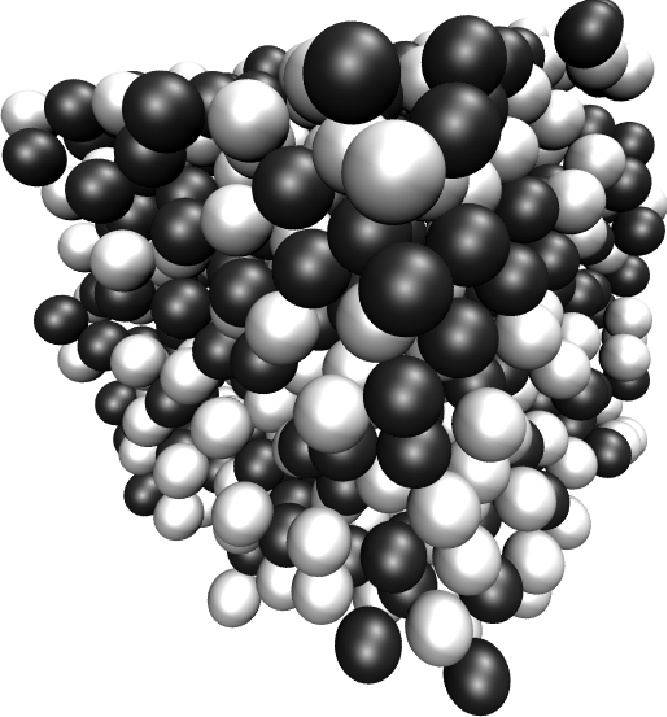
\includegraphics[width=0.4\textwidth]{figures/salt.png}
  \caption{VMD Snapshot of the salt system}
  \label{fig:snapshot}
\end{figure}

With these configurations, we can now investigate the system. As an example, we
will create a second script which calculates the averaged radial distribution
functions $g_{++}(r)$ and $g_{+-}(r)$. The radial distribution function for a
the current configuration can be obtained using the \verb|analyze| command:
\begin{tclcode}
set rdf [analyze rdf 0 1 0.9 [expr $box_l/2] 100]
set rlist ""
set rdflist ""
foreach value [lindex $rdf 1] {
  lappend rlist   [lindex $value 0]
  lappend rdflist [lindex $value 1] 
}
\end{tclcode}
The shown \verb|analyze rdf| command returns the distribution function of
particles of type 1 around particles of type 0 (i.~e.\ of opposite charges) for
radii between $0.9$ and half the box length, subdivided into $100$ bins.
Changing the first two parameters to either ``0 0'' or ``1 1'' allows to
determine the distribution for equal charges. The result is a list of $r$ and
$g(r)$ pairs, which the following foreach loop divides up onto two lists
\verb|rlist| and \verb|rdflist|.

To average over a set of configurations, we put the two last code snippets into
a loop like this:
\begin{tclcode}
set cnt 0
for {set i 0} {$i < 100} {incr i} { lappend avg_rdf 0}
foreach filename $argv {
  set f [open $filename "r"]
  while { [blockfile $f read auto] != "eof" } {}
  close $f
  set rdf [analyze rdf 0 1 0.9 [expr $box_l/2] 100]
  set rlist ""
  set rdflist ""
  foreach value [lindex $rdf 1] {
     lappend rlist   [lindex $value 0]
     lappend rdflist [lindex $value 1] }
  set avg_rdf [vecadd $avg_rdf $rdflist]
  incr cnt 
}
set avg_rdf [vecscale [expr 1.0/$cnt] $avg_rdf]
\end{tclcode}
Initially, the sum of all $g(r)$, which is stored in \verb|avg_rdf|, is set to
0.  Then the loops over all configurations given by \verb|argv|, calculates
$g(r)$ for each configuration and adds up all the $g(r)$ in \verb|avg_rdf|.
Finally, this sum is normalized by dividing by the number of
configurations. Note the ``1.0/\$cnt''; this is necessary, since ``1/\$cnt'' is
interpreted as an integer division, which results in 0 for $\text{cnt}>1$.
\verb|argv| is a predefined variable: it contains all the command line
parameters. Therefore this script should be called like
\begin{code}
Espresso \var{script} [\var{config}... ]
\end{code}

\begin{figure}[tb]
  \centering
  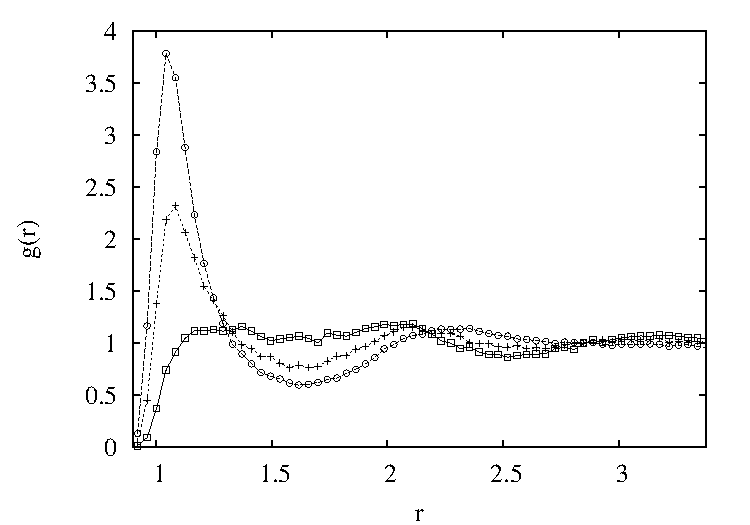
\includegraphics[width=0.7\textwidth]{figures/nacl-rdf.pdf}
  \caption{Radial distribution functions $g_{++}(r)$ between equal charges
    (rectangles) and $g_{+-}(r)$ for opposite charges (circles). The plus
    symbols denote $g(r)$ for an uncharged system.}
  \label{fig:rdf}
\end{figure}

The printing of the calculated radial distribution functions is simple. Add to the end of the
previous snippet the following lines:
\begin{tclcode}
set plot [open "rdf.data" "w"]
puts $plot "\# r rdf(r)"
foreach r $rlist rdf $avg_rdf { puts $plot "$r $rdf" }
close $plot
\end{tclcode}
This instructs the Tcl interpreter to write the \verb|avg_rdf| to the file \verb|rdf.data| in
gnuplot--compatible format. Fig.~\ref{fig:rdf} shows the resulting radial distribution functions,
averaged over 100 configurations. In addition, the distribution for a neutral
system is given, which can be obtained from our simulation script by simply
removing the command \verb|inter coulomb ...| and therefore not turning on P$^3$M.

The code example given before is still quite simple, and the reader is
encouraged to try to extend the example a little bit, e.~g. by using differently
sized particle, or changing the interactions. If something does not work, \es\
will give comprehensive error messages, which should make it easy to identify
mistakes. For real simulations, the simulation scripts can extend over thousands
of lines of code and contain automated adaption of parameters or online
analysis, up to automatic generation of data plots.  Parameters can be changed
arbitrarily during the simulation process, as needed for e.~g.\ simulated
annealing. The possibility to perform non--standard simulations without the need
of modifications to the simulation core was one of the main reasons why we
decided to use a script language for controlling the simulation core.

\section{\texttt{tutorial.tcl}}

In the directory \texttt{samples/} of the es{} sources, you will find
a well documented simulation script \texttt{tutorial.tcl}, which takes
you step by step through a slightly more complicated simulation of a
polyelectrolyte system. The basic structure of the script is however
the same as in the previous example and probably the same as the
structure of most \es{} simulation scripts.

Initially, some parameters and global variables are set, the
interactions are initialized, and particles are added. For this, the
script makes use of the \verb|polymer| command, which provides a
faster way to set up chain molecules.

The actual simulation falls apart again into two loops, the warmup
loop with increasing force capping, and the final simulation loop.
Note that the electrostatic interaction is only activated after
equilibrating the excluded volume interactions, which speeds up the
warmup phase. However, depending on the problem, this splitted warmup
may not be possible due to physical restrictions. \es{} cannot detect
these mistakes and it is your responsibility to find simulation
procedure suitable to your specific problem.

%%% Local Variables: 
%%% mode: latex
%%% TeX-master: "ug"
%%% End: 

\chapter{Compiling and installing \es}
\label{chap:install}
\index{Installation|textbf}

\begin{itemize}
\item Compiling \es{} is a necessary evil
\item Features can be compiled in or not
\item For maximal efficiency, compile in only the features that you
  use
\item \es{} can be obtained from the \es{} home page
  \footnote{\url{http://www.espresso.mpg.de}}.
\item If you are looking for the \es binary or the object files, read
  \vref{sec:builddir}
\item other than in most packages, \es will probably not be installed,
  or it will only be installed locally. Refer to \vref{sec:installdir}
  for details.
\end{itemize}

\section{Source and build directories}
\label{sec:builddir}
\index{build directory} \index{source directory}

Usually, when a program is compiled, the resulting binary files are
put into the same directory as the sources of the program. In \es, the
\emph{source directory} that contains all the source files is
completely separated from the \emph{build directory} where the files
created by the build process are put. As the source directory is not
modified during the compilation process, it is possible to compile more
than one binary versions of \es from a single set of source files.

The location of the build directory is determined when
\texttt{configure} is called.  Depending on whether it is called from
the source directory where it resides, or from some other directory,
the build system will act different.

When \texttt{configure} is called from another current working
directory than the source directory, this directory will become the
\emph{build directory}.  All files will be generated below the build
directory.  This way, you can make as many builds of \es as you like,
each build having different compiler flags and built-in features, and
for as many platforms as you want.  All further commands concerning
compiling and running \es{} have to be called from this directory,
instead of from the source directory.

When \texttt{configure} is called from the source directory where the
script resides, the \es build system has limited built-in capabilities
to handle different computer hardware.  A new subdirectory is created
in the source directory and \texttt{configure} is recursively called
from this directory, making the subdirectory the build directory.  The
directory is called \texttt{obj-}\textit{platform}\texttt{/}, where
\textit{platform} is an automatically determined descriptor of the CPU
type where the script was started, \eg
\mbox{\texttt{obj-Athlon\_64-pc-linux}}.  Note that this heuristic
will work in many cases, but it may not always work as intended.  When
you notice any problems, you can always call \texttt{configure} from
another directory.

In this case it is also possible to run the commands \texttt{make} and
\texttt{Espresso} directly in the source directory.  Furthermore, the
option \texttt{--enable-chooser} will be set in the recursive call of
\texttt{configure} that activates the automatic binary chooser (see
section \vref{sec:installdir}).

\paragraph{Example}
When the source directory is \texttt{\$srcdir} (\ie{} the files where
unpacked to this directory), then the build directory can be set to
\texttt{\$builddir} by calling the \texttt{configure}-script from
there:
\begin{code}
cd $builddir
$srcdir/configure
make
Espresso
\end{code}

\section{\texttt{myconfig.h}: Activating and deactivating features}
\label{sec:myconfig}

\index{features} \index{myconfig.h} \index{configuration header} \es
has a large number of features that can be compiled into the binary.
However, it is not recommended to actually compile in all possible
features, as this will negatively affect \es's performance.  Instead,
compile in only the features that are actually required.  For the
developers, it is also possible to turn on or off a number of
debugging messages.  The features and debug messages can be controlled
via a configuration header file that contains C-preprocessor
declarations. Appendix \vref{chap:features} lists and describes all
available features.  When no configuration header is provided by the
user, a default header will be used that turns on the default
features.  The file \texttt{myconfig-sample.h} in the source directory
contains a list of all possible features that can be copied into your
own configuration file.

When you distinguish between the build and the source directory (see
\vref{sec:builddir}), the configuration header can be put in either of
these. Note, however, that when a configuration header is found in
both directories, the one in the build directory will be used.  For an
example how this can be employed, see section \ref{sec:builddir}.

By default, the configuration header is called \texttt{myconfig.h}.
The name of the configuration header can be changed either when the
\texttt{configure}-script is called with the option
\mbox{\texttt{--with-myconfig}} (see section \vref{sec:configure}), or
when \texttt{make} is called with the setting
\mbox{\texttt{myconfig=}\textit{myconfig\_header}} (see section
\vref{sec:make}).

The configuration header can be used to compile different binary
versions of \es with a different set of features from the same source
directory.  Suppose that you have a source directory \texttt{\$srcdir}
and two build directories \texttt{\$builddir1} and
\texttt{\$builddir2} that contain different configuration headers:

\begin{itemize}
\item \texttt{\$builddir1/myconfig.h}:
\begin{code}
#define ELECTROSTATICS
#define LENNARD-JONES
\end{code}

\item \texttt{\$builddir2/myconfig.h}:
\begin{code}
#define LJCOS
\end{code}
\end{itemize}

\noindent Then you can simply compile two different versions of \es via
\begin{code}
cd $builddir1
$srcdir/configure
make

cd $builddir2
$srcdir/configure
make
\end{code}


\section{Running \texttt{configure}}
\label{sec:configure}

% Description of basic options: --prefix, --exec-prefix, CPPFLAGS,
% CFLAGS, LDFLAGS

\index{configure} The shell script \texttt{configure} collects all the
information required by the compilation process. It will determine how
to use and where to find the different libraries and tools required by
the compilation process, and it will test what compiler flags are to
be used.  The script will find out most of these things automatically.
If something is missing, it will complain and give hints how to solve
the problem.  The generic syntax of calling the \texttt{configure}
script is:
\begin{code}
configure [\var{options} ...] [\var{variable}=\var{value} ...]
\end{code}

\noindent Note that in the \es build system, the files generated by
the configuration and compilation process are not placed next to the
source files, but into a separate \emph{build directory} instead.
Refer to section \vref{sec:builddir} for details.

\index{configure options} The behaviour of \texttt{configure} can be
controlled by the means of command line options. In the following,
only those command line options that are specific to \es will be
explained.  For a complete list of options and explanations thereof,
call
\begin{code}
configure --help
\end{code}

\subsection{Options}

\begin{description}
\item [\texttt{--enable-chooser}] This option will enable the
  automatic binary chooser mechanism for \es (see section
  \vref{sec:installdir}).  This option will be automatically enabled,
  when the \texttt{configure} script is called from the source
  directory, otherwise it will be disabled. It is not recommended to
  set the option manually.
\item[\texttt{--enable-debug}] This option will enable compiler flags
  required for debugging the \es binary and is disabled by default.
\item[\texttt{--enable-profiling}] This option will enable compiler
  flags required for profiling the \es binary and is disabled by
  default.
\item[\texttt{--disable-processor-optimization}] This option will
  control whether \texttt{configure} will check for several
  optimization flags to be used by the compiler. This option is
  enabled by default.
\item[\texttt{--disable-xlc-qipa}] This option is only useful when the
  IBM C-compiler \texttt{xlc} is used and will control whether or not
  the compiler flag \texttt{-qipa} is used.  If you come upon problems
  when using the \es binary on IBM machines, try using
  \texttt{--disable-xlc-ipa}. The option is enabled by default.
\item[\texttt{--with-myconfig=MYCONFIG\_HEADER}] This option sets the
  name of the local configuration header (see \vref{sec:myconfig}). It
  defaults to ``\texttt{myconfig.h}''.
\item[\texttt{--with-mpi=MPI}/ \texttt{--without-mpi}] Sets the MPI
  implementation that should be used, or disables MPI. By default,
  \texttt{configure} will test automatically what MPI implementation
  is available. The following implementations are known:
  \begin{description}
  \item[\texttt{fake}, \texttt{no}] This will disable MPI
    completely. Equivalent to \mbox{\texttt{--without-mpi}}.
  \item[\texttt{lam}] Use the LAM/MPI environment
    (\url{http://www.lam-mpi.org/}).
  \item[\texttt{mpich}] Use the MPICH environment
    (\url{http://www-unix.mcs.anl.gov/mpi/mpich/}).
  \item[\texttt{poe}] Use the POE environment (IBM).
  \item[\texttt{dmpi}] Use the DMPI environment (Tru64).
  \item[\texttt{generic}] Use a generic MPI implementation. This will
    try to find an MPI compiler and an MPI runtime environment.
  \end{description}
\item[\texttt{--with-efence} / \texttt{--without-efence}] Whether or
  not to use the ``electric fence'' memory debugging library
  (\url{http://freshmeat.net/projects/efence/}). Efence is not used by
  default.
\item[\texttt{--with-tcl=TCL}] By default, \texttt{configure} will
  automatically determine which version of Tcl is used.  If the wrong
  version is chosen automatically, you can specify the name of the
  library with this option, \eg{} \texttt{tcl8.4}.
\item[\texttt{--with-tk=TK} / \texttt{--without-tk}] By default, the
  GUI toolkit Tk is not used by \es. This option can be used to
  activate Tk and to specify which Tk version to use, \eg{}
  \texttt{tk8.4}. If you only specify \texttt{--with-tk} and do not
  give a version number, \texttt{configure} will try to automatically
  deduce the right version.
\item[\texttt{--with-fftw=VERSION} / \texttt{--without-fftw}] This can
  be used to specify whether the FFTW library is to be used, and which
  version.  By default, version 3 will be used if it is found,
  otherwise version 2 is used.  Note that quite a number of central
  features of \es require FFTW.
\end{description}

\section{\texttt{make}: Compiling,  testing and installing \es}
\label{sec:make}

The command \texttt{make} is mainly used to compile the \es{} source
code, but it can do a number of other things. The generic syntax of
the \texttt{make} command is:
\begin{code}
make [\var{target}...] [\var{variable}=\var{value}]
\end{code}
When no target is given, the target \texttt{all} is used. The
following targets are available:
\begin{description}
\item[\texttt{all}] Compiles the complete \es source code. The
  variable \lit{myconf} can be used to specify the name of the
  configuration header to be used.
\item[\texttt{check}] Runs the testsuite. By default, all available
  tests will be run on 1, 2, 3, 4, 6, or 8 processors. Which tests are
  run can be controlled by means of the variable \texttt{tests}, which
  processor numbers are to be used can be controlled via the variable
  \texttt{processors}. Note that depending on your MPI installation,
  MPI jobs can only be run in the queueing system, so that \es{} will
  not run from the command line. In that case, you may not be able to
  run the testsuite, or you have to directly submit the testsuite script
  \verb!testsuite/test.sh! to the queueing system.\\
  \textbf{Example:} \verb!make check tests="madelung.tcl" processors="1 2"!\\
  will run the test \texttt{madlung.tcl} on one and two processors.
\item[\texttt{clean}] Deletes all files that were created during the
  compilation.
\item[\texttt{mostlyclean}] Deletes most files that were created
  during the compilation. Will keep for example the built doxygen
  documentation and the \es{} binary.
\item[\texttt{dist}] Creates a \texttt{.tar.gz}-file of the \es{}
  sources.  This will include all source files as they currently are
  in the source directory, \ie{} it will include local changes.  This
  is useful to give your version of \es{} to other people.
  The variable \texttt{extra} can be used to specify additional
  files and directories that are to be included in the archive
  file. \\
  \textbf{Example:} \verb!make dist extra="myconfig.h internal"!\\
  will create the archive file and include the file
  \texttt{myconfig.h} and the directory \texttt{internal} with all
  files and subdirectories.
\item[\texttt{install}] Install \es. The variables \texttt{prefix} and
  \texttt{exec-prefix} can be used to specify the installation
  directories, otherwise the defaults defined by the
  \texttt{configure} script are used. \texttt{prefix} sets the prefix
  where all \es files are to be installed, \texttt{exec-prefix} sets
  the prefix where the executable files are to be installed and is
  required only when there is an architecture-specific directory (\eg
  \texttt{/usr/local/bin64/}).  For the actual locations where the
  different files are installed, refer to section
  \vref{sec:installdir}.\\
  \textbf{Example:} \verb!make install prefix=/usr/local!\\
  will install all files below \texttt{/usr/local}.
\item[\texttt{uninstall}] Uninstalls \es{}, \ie{} removes all files
  that were installed during \texttt{make install}. The variables are
  identical to the variables of the \texttt{install}-target.
\end{description}

\subsection{Installation directories}
\label{sec:installdir}

\index{installation directory} Other than most software, \es is not
necessarily installed into the system, but can also be used directly
from the build directory.  The rest of this section is only
interesting if you plan to install \es.

Normally, the \es-binary \texttt{Espresso-bin} is installed in the
directory \texttt{\$prefix/libexec/} and a the wrapper script
\texttt{Espresso} in the directory \texttt{\$prefix/bin/} that handles
the MPI invocation.

When the \texttt{configure}-script is called from the source directory
or when the option \texttt{--enable-chooser} is given, an automatic
binary chooser is installed in the directory \texttt{\$prefix/bin/}
and the \es-binary and the MPI wrapper script are installed in an
architecture-specific subdirectory
\mbox{\texttt{\$exec-prefix/lib/espresso/obj-}\textit{platform}\texttt{/}}.
When called, the binary chooser will automatically call the MPI
wrapper script from the right subdirectory.

\section{Running \es}
\label{sec:run}

When \es is found in your path, it can be run via
\begin{code}
Espresso [\var{tcl\_script} [\var{N\_processors} [\var{args}]]]
\end{code}

\index{interactive mode} When \es{} is called without any arguments,
it is started in the interactive mode, where new commands can be
entered on the command line. When the name of a \textit{tcl\_script}
is given, the script is executed. \textit{N\_processors} is the number
of processors that are to be used. Any further arguments are passed to
the script. Note that depending on your MPI installation, MPI jobs can
only be run in the queueing system, so that \es will not run from
the command line.

% A number of wrapper scripts are used in running \es{}:
% \begin{itemize}
% \item The script \texttt{Espresso} in the source and build directory
%   will try to run the compiled version of \es. If it is called from
%   the source directory, it assumes that \es{} was also configured in
%   the source directory and will try to recursively start the script in
%   the corresponding \texttt{obj-PLATFORM} build directory. If it is
%   called in the build directory, it will start the \es-binary with the
%   right MPI implementation.
% \item The chooser script \texttt{Espresso} 
%   \begin{itemize}
%   \item installed when \verb!--enable-chooser! was given
%   \item installed to bindir
%   \item tries to run the correct version of the MPI-wrapper
%     \texttt{Espresso}
%   \end{itemize}
% \item The MPI-wrapper \texttt{Espresso}
%   \begin{itemize}
%   \item installed next to \es{} binary
%   \item starts the binary with the right MPI implementation
%   \end{itemize}
% \item The \es{} binary \texttt{Espresso-bin} can also be started
%   directly, however, it requires that the environment variable
%   \verb!ESPRESSO_SCRIPTS! is set to the directory where the scripts
%   are installed (usually \verb!$(prefix)/lib/espresso/scripts! or
%   \verb!$(prefix)/share/espresso/scripts!).
% \end{itemize}


%%% Local Variables: 
%%% mode: latex
%%% TeX-master: "ug"
%%% End: 

\chapter{Setting up the system}
\label{chap:setup}

\section{\texttt{setmd}: Setting global variables.}
\newescommand{setmd}

\begin{essyntax}
\variant{1} setmd \var{variable}
\variant{2} setmd \var{variable} \opt{\var{value}}+
\end{essyntax}
\todo{Explain '+' in intro.}

Variant \variant{1} returns the value of the \es global variable
\var{variable}, variant \variant{2} can be used to set the variable
\var{variable} to \var{value}. The following global variables can be
set:

%% List-environment for the description of the global variables
\newenvironment{globvar}{
  \begin{list}{}{
      \setlength{\rightmargin}{1em}
      \setlength{\leftmargin}{2em}
      \setlength{\partopsep}{0pt}
      \setlength{\topsep}{1ex}
      \setlength{\parsep}{0.5ex}
      \setlength{\listparindent}{-1em}
      \setlength{\labelwidth}{0.5em}
      \setlength{\labelsep}{0.5em}
      \renewcommand{\makelabel}[1]{%
        \index{##1@\texttt{##1} (global variable)|mainindex}%
        \index{global variables!\texttt{##1}|mainindex}%
        \texttt{##1}%
      }
    }
  }{
  \end{list}
}
\newcommand{\ro}{\emph{read-only}}

\todo{Better throw some out (\eg switches)?}
\todo{Missing: lattice_switch, dpd_tgamma, n_rigidbonds}
\todo{Which commands can be used to set the \emph{read-only}
  variables?}
\begin{globvar}
\item[box_l] (double[3]) Simulation box length.
  \todo{document what happens to the particles when \keyword{box_l} is
    changed!}
\item[cell_grid] (int[3], \ro) Dimension of the inner
  cell grid.
\item[cell_size] (double[3], \ro) Box-length of a cell.
\item[dpd_gamma] (double, \ro) Friction constant for the
  DPD thermostat.
\item[dpd_r_cut] (double, \ro) Cutoff for DPD thermostat.
\item[gamma] (double, \ro) Friction constant for the
  Langevin thermostat.
\item[integ_switch] (int, \ro) Internal switch which integrator to
  use.
\item[local_box_l] (int[3], \ro) Local simulation box length of the
  nodes.
\item[max_cut] (double, \ro) Maximal cutoff of real space
  interactions.
\item[max_num_cells] (int) Maximal number of cells for the link cell
  algorithm.  Reasonable values are between 125 and 1000, or for some
  problems (\var{n_total_particles} / \var{n_nodes}).
\item[max_part] (int, \ro) Maximal identity of a particle.
  \emph{This is in general not related to the number of particles!}
\item[max_range] (double, \ro) Maximal range of real space
  interactions: \var{max_cut} + \var{skin}.
\item[max_skin] (double, \ro) Maximal skin to be used for the link
  cell/verlet algorithm. This is the minimum of \var{cell_size} -
  \var{max_range}. \todo{???}
\item[min_num_cells] (int) \todo{???} Minimal number of cells for the
  link cell algorithm. Reasonable values range in $1e-6 N^2$ to $1e-7
  N^2$. In general just make sure that the Verlet lists are not
  incredibly large. By default the minimum is 0, but for the automatic
  P3M tuning it may be wise to larger values for high particle
  numbers.
\item[n_layers] (int, \ro) Number of layers in cell structure LAYERED
  (see section \vref{sec:cell-systems}).
\item[n_nodes] (int, \ro) Number of nodes.
\item[n_part] (int, \ro) Total number of particles.
\item[n_part_types] (int, \ro) Number of particle types that were
  used so far in the \keyword{inter} command (see chapter{tcl:inter}).
\item[node_grid] (int[3]) 3D node grid for real space domain
  decomposition (optional, if unset an optimal set is chosen
  automatically).
\item[nptiso_gamma0] (double, \ro)\todo{Docs missing.}
\item[nptiso_gammav] (double, \ro)\todo{Docs missing.}
\item[npt_p_ext] (double, \ro) Pressure for NPT simulations.
\item[npt_p_inst] (double) Pressure calculated during an
  NPT_isotropic integration.
\item[piston] (double, \ro) Mass off the box when using NPT_isotropic
  integrator.
\item[periodicity] (bool[3]) Specifies periodicity for the three
  directions. If the feature PARTIAL_PERIODIC is set, this variable
  can be set to (1,1,1) or (0,0,0) at the moment.  If not it is
  readonly and gives the default setting (1,1,1).\todo{Correct?}
\item[skin] (double) Skin for the Verlet list.
\item [temperature] (double, \ro) Temperature of the
  simulation.
\item[thermo_switch] (double, \ro) Internal variable which thermostat
  to use. 
\item[time] (double) The simulation time.
\item[time_step] (double) Time step for MD integration.
\item[timings] (int) Number of timing samples to take into account if
  set.\todo{???}
\item[transfer_rate] (int, \ro) Transfer rate for VMD connection. You
  can use this to transfer any integer value to the simulation from
  VMD.
\item[verlet_flag] (bool) Indicates whether the Verlet list will be
  rebuild. The program decides this normally automatically based on
  your actions on the data.
\item[verlet_reuse] (double) Average number of integration steps the
  verlet list has been re-used.
\end{globvar}

\section{\texttt{thermostat}: Setting up the thermostat}
\newescommand{thermostat}

\begin{essyntax}
  \variant{1} thermostat off
  \variant{2} theormstat \var{method} \opt{\var{parameter}}+
\end{essyntax}
\todo{Include docs from \texttt{thermostat.h}!}
Change thermostat settings.

\section{\texttt{nemd}: Setting up non-equilibrium MD}
\newescommand{nemd}

\begin{essyntax}
  \variant{1}nemd \var{method} \var{parameter} 
  \variant{2}nemd off
  \variant{3}nemd profile
  \variant{4}nemd viscosity
\end{essyntax}
\todo{Include docs from \texttt{nemd.h}!}
\todo{Put \texttt{nemd profile|viscosity} into \texttt{analyze}?}  
Use NEMD (Non Equilibrium Molecular Dynamics) to simulate a system
under shear.

\section{\texttt{cellsystem}: Setting up the cell system}
\label{sec:cell-systems}
\newescommand{cellsystem}

This section deals with the flexible particle data organization of
\es.  Due to different needs of different algorithms, \es is able to
change the organization of the particles in the computer memory,
according to the needs of the used algorithms. For details on the
internal organization, refer to section
\vref{sec:internal-particle-organization}.

\subsection{Domain decomposition}
\index{domain decomposition}
\begin{essyntax}
  cellsystem domain_decomposition \opt{-no_verlet_list}
\end{essyntax}
This selects the domain decomposition cell scheme, using Verlet lists
for the calculation of the interactions. If you specify
\keyword{-no_verlet_list}, only the domain decomposition is used, but
not the Verlet lists.

The domain decomposition cellsystem is the default system and suits
most applications with short ranged interactions. The particles are
divided up spatially into small compartments, the cells, such that the
cell size is larger than the maximal interaction range. In this case
interactions only occur between particles in adjacent cells. Since the
interaction range should be much smaller than the total system size,
leaving out all interactions between non-adjacent cells can mean a
tremendous speed-up. Moreover, since for constant interaction range,
the number of particles in a cell depends only on the density. The
number of interactions is therefore of the order N instead of order
$N^2$ if one has to calculate all pair interactions.

\subsection{N-squared}
\begin{essyntax}
  cellsystem nsquare 
\end{essyntax}
This selects the very primitive nsquared cellsystem, which calculates
the interactions for all particle pairs. Therefore it loops over all
particles, giving an unfavorable computation time scaling of $N^2$.
However, algorithms like MMM1D or the plain Coulomb interaction in the
cell model require the calculation of all pair interactions.

In a multiple processor environment, the nsquared cellsystem uses a
simple particle balancing scheme to have a nearly equal number of
particles per CPU, \ie $n$ nodes have $m$ particles, and $p-n$ nodes
have $m+1$ particles, such that $n*m+(p-n)*(m+1)=N$, the total number
of particles. Therefore the computational load should be balanced
fairly equal among the nodes, with one exception: This code always
uses one CPU for the interaction between two different nodes. For an
odd number of nodes, this is fine, because the total number of
interactions to calculate is a multiple of the number of nodes, but
for an even number of nodes, for each of the $p-1$ communication
rounds, one processor is idle.

E.g. for 2 processors, there are 3 interactions: 0-0, 1-1, 0-1.
Naturally, 0-0 and 1-1 are treated by processor 0 and 1, respectively.
But the 0-1 interaction is treated by node 1 alone, so the workload
for this node is twice as high. For 3 processors, the interactions are
0-0, 1-1, 2-2, 0-1, 1-2, 0-2. Of these interactions, node 0 treats 0-0
and 0-2, node 1 treats 1-1 and 0-1, and node 2 treats 2-2 and 1-2.

Therefore it is highly recommended that you use nsquared only with an
odd number of nodes, if with multiple processors at all. 

\subsection{Layered cell system}
\begin{essyntax}
  cellsystem layered \var{n_layers}
\end{essyntax}

This selects the layered cell system, which is specifically designed
for the needs of the MMM2D algorithm. Basically it consists of a
nsquared algorithm in x and y, but a domain decomposition along z, i.
e. the system is cut into equally sized layers along the z axis. The
current implementation allows for the cpus to align only along the z
axis, therefore the processor grid has to have the form 1x1xN.
However, each processor may be responsible for several layers, which
is determined by \var{n\_layers}, i. e. the system is split into
N*\var{n\_layers} layers along the z axis. Since in x and y direction
there are no processor boundaries, the implementation is basically
just a stripped down version of the domain decomposition cellsystem.

%%% Local Variables: 
%%% mode: latex
%%% TeX-master: "ug"
%%% End: 

\chapter{Running the simulation}
\label{chap:run}

\section{\texttt{integrate}: Running the simulation}
\eslabel{integrate}

\begin{essyntax}
  \variant{1} integrate \var{steps}
  \variant{2} integrate set \var{method} \opt{\var{parameter}}+
\end{essyntax}

\todo{Docs missing!}
\todo{Which integrators do exist?}

\section{\texttt{change_volume}: Changing the box volume}
\eslabel[change-volume]{change_volume}

\begin{essyntax}
  \variant{1} change_volume \var{V_new} 
  \variant{2} change_volume \var{L_new} \alt{x \asep y \asep z \asep xyz}
\end{essyntax}
Changes the volume of either a cubic simulation box to the new volume
\var{V_new} or its given x-/y-/z-/xyz-extension to the new box-length
\var{L_new}, and isotropically adjusts the particles coordinates as
well. The function returns the new volume of the deformed simulation
box.

\section{Stopping particles}
\eslabel{stopParticles}
\eslabel[stop-particles]{stop_particles}

\begin{essyntax}
  \variant{1} stopParticles
  \variant{2} stop_particles
\end{essyntax}
Halts all particles in the current simulation, setting their
velocities and forces to zero. Variant \variant{2} does not provide
feedback on the execution status.

\section{\texttt{velocities}: Setting the velocities}
\eslabel{velocities}
\begin{essyntax}
  velocities \var{v_max} 
  \opt{start \var{part_id}} 
  \opt{count \var{N_T}}
\end{essyntax}
Sets the velocities of the particles with particle ID (see The part
command) between \var{part_id} and \var{part_id}+\var{N_T}
(defaults to '0' \& '[setmd npart]-\var{part_id}') to a random vector
with length in [-vmax,vmax], and returns the absolute value of the
total velocity assigned.

\section{\texttt{invalidate_system}}
\eslabel[invalidate-system]{invalidate_system}
\begin{essyntax}
  invalidate_system
\end{essyntax}
\todo{Documentation not up to date!}

Forces a system re-init which, among others, causes the integrator to
also update the forces at its beginning (instead of re-using the
values from the previous integration step).  This is particularly
necessary to ensure continuity after setting a checkpoint:
\texttt{integrate} - \texttt{set_checkpoint} - \texttt{integrate} has
only one call to \todo{???}???, while \texttt{read_checkpoint} -
\texttt{integrate} has two at the beginning of the 2nd integrate
(because loading a new system from disk typically requires
re-initializing the system), and since ??? also uses the thermostat
which in turn draws random numbers, the two situations do not end up
at the same segment of the random number sequence, all random events
will therefore slightly differ.  To prevent this, simply include a
call to invalidate_system upon setting the checkpoint (this is being
done automatically if using tcl_checkpoint_set and
tcl_checkpoint_read beginning with v1.1 of \es{}), because in that
case both scenarios will call ??? twice at the beginning of the second
integration phase thus having their random number sequences in total
sync. The C implementation is invalidate_system.



%%% Local Variables: 
%%% mode: latex
%%% TeX-master: "ug"
%%% End: 

\chapter{Analysis}
\label{chap:analysis}


%%% Local Variables: 
%%% mode: latex
%%% TeX-master: "ug"
%%% End: 

\chapter{Auxilliary commands}
\label{chap:aux}

\section{Writing VTF files}
%\quickrefheading{Handling of VTF files}

There are two commands in \es{} that support writing files in the VMD
formats VTF, VSF and VCF.\footnote{A description of the format and a
  plugin to read the format in VMD is found in the subdirectory
  \texttt{vmdplugin/} of the \es{} source directory.} The commands can
be used to write the structure (\texttt{writevsf}) and coordinates
(\texttt{writevcf}) of the system to a single trajectory file (usually
with the extension \texttt{.vtf}), or to separate files (extensions
\texttt{.vsf} and \texttt{.vtf}).

\subsection{\texttt{writevsf}}

\tclcommand{writevsf}
{\var{file} [<short|verbose>] [<\var{radii}|auto>] [typedesc \var{typedesc}]}

Writes a structure block describing the system's structure to
\var{file}. The atom ids used in the file are identical to \es's
particle ids.  This makes it easy to write additional structure lines
to the file, e.g. to specify the \texttt{resname} of particle
compounds, like chains.  The output of this file can be used in a
standalone VSF file, or at the beginning of a trajectory VTF file that
contains a trajectory of a whole simulation.

\begin{tcloptions}
  \option{<short|verbose>}
  Specify, whether the output is in a human-readable, but somewhat
  longer format (\keyword{verbose}), or in a more compact form
  (\keyword{short}). The default is \keyword{verbose}.
  
  \option{<radius \var{radii}|auto>}
  Specify the VDW radii of the atoms. \var{radii} is either
  \keyword{auto}, or a Tcl-list describing the radii of the different
  particle types. When the keyword \keyword{auto} is used and a
  Lennard-Jones interaction between two particles of the given type is
  defined, the radius is set to be $\frac{\sigma_{LJ}}{2}$ plus the LJ
  shift.  Otherwise, the radius $0.5$ is substituted. The default is
  \keyword{auto}.
  
  Example: \verb!writevsf "show.tcl" radius {{0 2.0} {1 auto} {2 1.0}}!
  
  \option{typedesc \var{typedesc}}
  \var{typedesc} is a Tcl-list giving additional VTF atom-keywords to
  specify additional VMD characteristics of the atoms of the given type.
  If no description is given for a certain particle type, it defaults to
  \texttt{segid \textit{n}}, where \textit{n} is the type id.

  Example: \verb!writevsf "show.tcl" typedesc {{0 "segid colloid"} {1 "segid pe"}}!
\end{tcloptions}


\subsection{\texttt{writevcf}}
\tclcommand{writevcf}
{\var{file} [<short|verbose>] [<folded|absolute>]}

Writes a coordinate (or timestep) block that contains all coordinates
of the system's particles to \var{file}.

\begin{tcloptions}
  \option{<short|verbose>} Specify, whether the output is in a
  human-readable, but somewhat longer format (\keyword{verbose}), or
  in a more compact form (\keyword{short}). The default is
  \keyword{verbose}.

  \option{<folded|absolute>} Specify whether the particle positions
  are written in absolute coordinates (\keyword{absolute}) or folded
  into the central image of a periodic system (\keyword{folded}). The
  default is \keyword{absolute}.

  \option{<pids \var{pids}|all>} Specify the coordinates of which particles
  should be written. If \keyword{all} is used, all coordinates will be
  written (in the ordered timestep format). Otherwise, \var{pids} has
  to be a Tcl-list specifying the pids of the particles. The default
  is \keyword{all}.
  
  Example: \verb!pids {0 23 42}!

\end{tcloptions}


%%% Local Variables: 
%%% mode: latex
%%% TeX-master: "ug"
%%% End: 

\chapter{Under the hood}
\label{chap:underhood}

(new)

\begin{itemize}
\item Implementation issues that are interesting for the user
\item Main loop in pseudo code (for comparison)
\item from doxygen: ``Cell systems'' 
\end{itemize}

%%% Local Variables: 
%%% mode: latex
%%% TeX-master: "ug"
%%% End: 

\chapter{Getting involved}
\label{chap:devel}

\begin{itemize}
\item What to do when you want to become involved
\item How to submit a bug report
\item Reference to developer's guide
\end{itemize}

%%% Local Variables: 
%%% mode: latex
%%% TeX-master: "ug"
%%% End: 


\appendix
\chapter{\es{} quick reference}
\label{chap:quickref}

\index{quick reference of Tcl-commands}
%\documentclass[
a4paper,                        % paper size
11pt,                           % font size
twoside,                        % two sided
footsepline,                    % add a line to separate the footer
headsepline,                    % add a line to separate the header
headexclude,                    % header does not belong to the text
footexclude,                    % footer does not belong to the text
pagesize,                       % set the pagesize in a DVI document
bibtotocnumbered,               % add the bibliography to the TOC
idxtotoc                        % add the index to the TOC
%openright,                      % start a new chapter on the right page
%,DIV12
%,draft
]{scrreprt}

\usepackage{nameref}            % nameref, varioref, hyperref must be
                                % used in this order (see hyperref
                                % README)!
\usepackage[draft]{varioref}    % defines \vref
\usepackage[bookmarksopen=true]
{hyperref}                      % automatically creates links when
                                % using pdflatex, defines \url
\usepackage{ifpdf}              % defines \ifpdf
\usepackage{graphicx}           % handles graphics
\usepackage{makeidx}            % creates the index
\usepackage{color}              % use colors

\usepackage{verbatim}           % required for \verbatim and \endverbatim
\usepackage{alltt}              % almost verbatim environment (code)
\usepackage{tocloft}            % required for the quickref
\usepackage{calc}               % compute length
\usepackage{ifthen}             % provide ifthen

%%%%%%%%%%%%%%%%%%%%%%%%%%%%%%%%%%%%%%%%%%%%%%%%%%
%%%%%%%%%%%%%%%%%%%%%%%%%%%%%%%%%%%%%%%%%%%%%%%%%%
%%%%%%%%% New Commands and Environments %%%%%%%%%%
%%%%%%%%%%%%%%%%%%%%%%%%%%%%%%%%%%%%%%%%%%%%%%%%%%
%%%%%%%%%%%%%%%%%%%%%%%%%%%%%%%%%%%%%%%%%%%%%%%%%%
\newcommand{\es}{\mbox{\textsf{ESPResSo}}}
\newcommand{\ie}{\textit{i.e.\/}}
\newcommand{\eg}{\textit{e.g.\/}}
\newcommand{\etal}{\textit{et al.\/}}

\newcommand{\codebox}[1]%
{%
  \begingroup\setlength{\fboxsep}{1pt}%
  \fcolorbox[rgb]{0,0,0}{0.9,0.9,0.9}{\ttfamily#1}%
  \endgroup%
}

\newsavebox{\thecodebox}
\newenvironment{code}{
  \begin{lrbox}{\thecodebox}
    \begin{minipage}{\linewidth-2em}
      \begin{alltt}
      }{
      \end{alltt}
    \end{minipage}
  \end{lrbox}
  \smallskip
  \begin{addmargin}[1em]{0pt}
    \codebox{\usebox{\thecodebox}}
  \end{addmargin}
  \smallskip
}

\makeatletter
\newenvironment{tclcode}
{
  \addtolength{\linewidth}{-2em}% set the line length
  \@minipagetrue%%%DPC%%%
  \@tempswatrue%%%DPC%%%
  \hsize=\linewidth%
  \setbox0=\vbox\bgroup\verbatim
}{\endverbatim
  \unskip\setbox0=\lastbox%%%DPC%%%
  \egroup
  \par
  \smallskip
  \noindent
  \begin{addmargin}[1em]{0pt}
    \codebox{\box0}
  \end{addmargin}
  \par
  \smallskip
  \noindent
}
\makeatother


%%%%%%%%%%%%%% Syntax Description %%%%%%%%%%%%%%%

%%%%%% SYNTAX DEFININTION LAYOUT
% typesetting inside a command definition
% keywords/literals
\newcommand{\lit}[1]{\mbox{\texttt{#1}}}
\newcommand{\keyword}[1]{\mbox{\texttt{#1}}}
% variables
\newcommand{\var}[1]{\mbox{\textrm{\textit{#1}}}}
% option
\newcommand{\opt}[1]{\mbox{[#1]}}

% command definition
\newcommand{\tclcommand}[3][]{%
  \stepcounter{qrfcounter}
  \index{#2@\texttt{#2}|textbf}
  \index{Tcl-commands!#2@\texttt{#2}|textbf}
  \addtocontents{qrf}{\protect\qrfcommand{#1}{#2}{#3}{\thepage}{qrf\alph{qrfcounter}}}
  \minisec{Syntax}
  \smallskip
  \hypertarget{qrf\alph{qrfcounter}}{%
    \codebox{%
      #2
      \parbox[t]{0.9\linewidth-\widthof{#2}}%
      {\ttfamily\raggedright\mbox{}#3}
    }%
  }%
  \ifthenelse{\equal{#1}{}}{}{%
    \minisec{Required features}
    \texttt{#1}
  }
  \minisec{Description}
}


\newenvironment{arguments}{
  \minisec{Arguments}
  \begin{list}{}{
      \setlength{\rightmargin}{1em}
      \setlength{\leftmargin}{2em}
      \setlength{\partopsep}{0pt}
      \setlength{\topsep}{1ex}
      \setlength{\parsep}{0.5ex}
      \setlength{\listparindent}{1em}
      \setlength{\labelwidth}{0.5em}
      \setlength{\labelsep}{0.5em}
      \renewcommand{\makelabel}[1]{\codebox{##1}}
    }
  }{
  \end{list}
}

\newcommand{\addtoquickref}[1]{\addtocontents{qrf}{#1}}
\newcommand{\quickrefheading}[1]{%
  \stepcounter{qrfcounter}
  \addtocontents{qrf}{\protect\qrfheading{#1}{\thepage}{qrf\alph{qrfcounter}}}
  \hypertarget{qrf\alph{qrfcounter}}{}
}


%%%%% QUICK REFERENCE LAYOUT
% Create quick reference list
\newlistof{commands}{qrf}{}
\newcommand{\qrflastpage}{} % save the last page number
\newcounter{qrfcounter} % the current number of the cmd

\makeatletter
\newcommand{\qrfheading}[3]{
  \@dottedtocline{1}{0pt}{0pt}{\hyperlink{#3}{\textsf{\textbf{#1}}}}{#2}
  \renewcommand{\qrflastpage}{#2}%
}
\makeatother

% command definition in the quickref
\newcommand{\qrfcommand}[5]{%
  \begin{addmargin}[1em]{0pt}%
    \hyperlink{#5}{%
      \ttfamily
      #2
      \parbox[t]{0.9\linewidth-\widthof{#2}}%
      {\raggedright #3}%
    }%
  % print the page number if it is differnet from the last entry
    \ifthenelse{\equal{\qrflastpage}{#4}}{}{\hfill\scriptsize #4}%
    \ifthenelse{\equal{#1}{}}{}{%
      \scriptsize\\\hspace*{1em} Required features: \texttt{#1}%
    }%
  \end{addmargin}%
  \ifthenelse{\equal{\qrflastpage}{#4}}{}{\renewcommand{\qrflastpage}{#4}}%
  \smallskip
}



%%%%%%%%%%%%%%%%%%%%%%%%%%%%%%%%%%%%%%%%%%%%%%%%%%
%%%%%%%%%%%%%%%%%%%%%%%%%%%%%%%%%%%%%%%%%%%%%%%%%%
%%%%%%%%%%%%%%%% Other Settings %%%%%%%%%%%%%%%%%%
%%%%%%%%%%%%%%%%%%%%%%%%%%%%%%%%%%%%%%%%%%%%%%%%%%
%%%%%%%%%%%%%%%%%%%%%%%%%%%%%%%%%%%%%%%%%%%%%%%%%%
\pagestyle{headings}
\makeindex

%%%%%%%%%%%%%%%%%%%%%%%%%%%%%%%%%%%%%%%%%%%%%%%%%%
%%%%%%%%%%%%%%%%%%%%%%%%%%%%%%%%%%%%%%%%%%%%%%%%%%
%%%%%%%%%%%%%%%%% Main Document %%%%%%%%%%%%%%%%%%
%%%%%%%%%%%%%%%%%%%%%%%%%%%%%%%%%%%%%%%%%%%%%%%%%%
%%%%%%%%%%%%%%%%%%%%%%%%%%%%%%%%%%%%%%%%%%%%%%%%%%
\begin{document}
\titlehead{
  \begin{center}
    
\includegraphics[width=5cm]{figures/logo}
  \end{center}
}
%\subject{}
\title{\es{} User's Guide}
%\author{}
%\date{\today}
\maketitle

\pdfbookmark{Contents}{toc}
\tableofcontents

\chapter{Introduction}
\label{chap:intro}

\todo{Make the following lists full text.}

\begin{itemize}
\item \es{} is a generic soft matter simulation packages
\item for molecular dynamics simulations in soft matter research
\item focussed on coarse-grained models
\item employs modern algorithms (Lattice-Boltzmann, DPD, P3M, \ldots)
\item written in C for maximal portability
\item Tcl-controlled
\item parallelized
\end{itemize}

\section{Guiding principles}
\label{sec:ideas}

(from paper: 2.1 Goals and principles)

\es
\begin{itemize}
\item does \emph{not} do the physics for you!
\item requires you to understand what you do (can not be used as a
  black box)
\item gives you maximal freedom (flexibility)
\item is extensible
\item integrates system setup, simulation and analysis, as this can't
  be strictly separated in soft matter simulations
\item has no predefined units
\item sets as few defaults as possible
\end{itemize}

\section{Algorithms contained in \es}

The following algorithms are implemented in \es{}:

\begin{itemize}
\item ensembles: NVE, NVT, NpT
\item charged systems:
  \begin{itemize}
  \item P3M for fully periodic systems
  \item ELC and MMM-family of algorithms for charged systems with
    non-periodic boundary conditions
  \item Maggs algorithm 
  \end{itemize}
\item Hydrodynamics:
  \begin{itemize}
  \item DPD (as a thermostat)
  \item Lattice-Boltzmann
  \end{itemize}
\end{itemize}

\section{Basic program structure}
\label{sec:structure}

(from paper: 2.2 Basic program structure)

\begin{itemize}
\item Control level: \texttt{Tcl}
\item ``Kernel'' written in \texttt{C}
\item This user's guide will focus on the control level
\end{itemize}

\section{On units}
\label{sec:units}
\index{units}
\index{length unit}
\index{time unit}
\index{energy unit}
\index{physical units}

What is probably one of the most confusing subjects for beginners of
\es is, that \es does not predefine any units.  While most MD programs
specify a set of units, like, for example, that all lengths are
measured in \AA ngstr\"om or nanometers, times are measured in nano- or
picoseconds and energies are measured in $\frac{kJ}{\mathrm{mol}}$,
\es does not do so.

Instead, the length-, time- and energy scales can be freely chosen by
the user.  A length of $1.0$ can mean a nanometer, an \AA ngstr\"om,
or a kilometer - depending on the physical system, that the user has
in mind when he writes his \es-script.  The user can choose the unit
system that suits the system best.

When creating particles that are intended to represent a specific type
of atoms, one will probably use a length scale of \AA ngstr\"om.  This
would mean, that \eg the parameter $\sigma$ of the Lennard-Jones
interaction between two atoms would be set to twice the van-der-Waals
radius of the atom in \AA ngstr\"om.  Alternatively, one could set
$\sigma$ to $2.0$ and measure all lengths in multiples of the
van-der-Waals radius.

The second choice to be made is the energy (and time-) scale.  One can
for example choose to set the Lennard-Jones parameter $\epsilon$ to
the energy in $\frac{kJ}{\mathrm{mol}}$.  Then all energies will be
measured in that unit.  Alternatively, one can choose to set it to
$1.0$ and measure everything in multiples of the van-der-Waals binding
energy.

As long as one remains within the same unit system throughout the
whole \es-script, there should be no problems.

\section{Requirements}
\label{sec:requirements}
\index{requirements}

The following libraries and tools are required to be able to compile
and use \es:

\begin{description}
\item[Tcl/Tk] \index{Tcl/Tk} \es{} requires the Toolkit Command
  Language Tcl/Tk \footnote{\url{http://www.tcl.tk/}} in the version
  8.3 or later.  Some example scripts will only work with Tcl 8.4. You
  do not only need the interpreter, but also the header files and
  libraries.  Depending on the operating system, these may come in
  separate development packages. If you want to use a graphical user
  interface (GUI) for your simulation scripts, you will also need Tk.
  
\item[FFTW] \index{FFTW} In addition, \es{} needs the FFTW library
  \footnote{\url{http://www.fftw.org/}} for Fourier transforms.
  ESPResSo can work with both the 2.1.x and 3.0.x series. Again, the
  header files are required.
  
\item[MPI] \index{MPI} Finally, if you want to use \es{} in parallel,
  you need a working MPI environment (version 1.2). Currently, the
  following MPI implementations are supported:
  \begin{itemize}
  \item LAM/MPI is the preferred variant
  \item MPICH, which seems to be considerably slower than LAM/MPI in
    our benchmarks.
  \item On AIX systems, \es{} can also use the native POE parallel
    environment.
  \item On DEC/Compaq/HP OSF/Tru64, \es{} can also use the native
    dmpirun MPI environment.
  \end{itemize}
\end{description}


\section{Syntax description}
\label{sec:syntax}


Throughout the user's guide, formal definitions of the syntax of
several Tcl-commands can be found. The following conventions are used
in these decriptions:
\begin{itemize}
\item Different \emph{variants} of a command are labelled \variant{1},
  \variant{2}, \ldots
\item Keywords and literals of the command that have to be typed
  exactly as given are written in \lit{typewriter} font.
\item If the command has variable arguments, they are set in
  \var{italic font}. The description following the syntax definition
  should contain a detailed explanation of the argument and its
  type.
\item \texttt{\alt{\var{alt1} \asep \var{alt2}}} specifies, that one
  of the alternatives \var{alt1} or \var{alt2} can be used.
\item \texttt{\opt{\var{argument}}} specifies, that the arugment
  \var{argument} is optional, \ie{} it can be omitted.
\item When an optional argument or a whole command is marked by a
  superscript label (\fmark{1}), this denotes that the argument can
  only be used, when the corresponding feature (see appendix
  \vref{chap:features}) specified in ``Required features'' is
  activated.
\end{itemize}


\minisec{Example}

\renewcommand{\variant}[1]{\par\rawvariant{#1}}
\begin{essyntaxbox}
  \variant{1} 
  constraint wall normal \var{n_x} \var{n_y} \var{n_z} 
  dist \var{d} type \var{id}
  
  \variant{2}
  constraint sphere center \var{c_x} \var{c_y} \var{c_z} 
  radius \var{rad} direction \var{direction} type \var{id} 
  
  \require{1}{%
    \variant{3}
    constraint rod center \var{c_x} \var{c_y} 
    lambda \var{lambda}
  } 
  
  \require{2,3}{%
    \variant{4}
    constraint ext_magn_field \var{f_x} \var{f_y} \var{f_z} 
  }

  \begin{features}
    \required{CONSTRAINTS}
    \required[1]{ELECTROSTATICS}
    \required[2]{ROTATION}
    \required[3]{DIPOLES}
  \end{features}

\end{essyntaxbox}
\renewcommand{\variant}[1]{\rawvariant{#1}}

%%% Local Variables: 
%%% mode: latex
%%% TeX-master: "ug"
%%% End: 


\chapter{First steps}
\label{chap:firststeps}

\section{Quick installation}

\index{configure}\index{make}

If you have the requirements (see section \vref{sec:requirements})
installed, in many cases, to compile \es{}, it is enough to execute
the following sequence of two steps in the directory where you have
unpacked the sources:
\begin{code}
configure
make
\end{code}

\todo{Mention minimal configuration without myconfig.h}
In some cases, \eg{} when \es{} needs to be compiled for several
different platforms or when different versions with different sets of
features are required, it might be useful to execute the commands not
in the source directory itself, but to start \texttt{configure} from
another directory (see section \vref{sec:builddir}). Furthermore, many
features of \es{} can be selectively turned on or off in the local
configuration header of \es{} (see section \vref{sec:myconfig}) before
starting the compilation with \texttt{make}.

The shell script \texttt{configure} prepares the source code for
compilation. It will determine how to use and where to find the
different libraries and tools required by the compilation process, and
it will test what compiler flags are to be used.  The script will find
out most of these things automatically.  If something is missing, it
will complain and give hints how to solve the problem.  The
configuration process can be controlled with the help of a number of
options that are explained in section \vref{sec:configure}.

The command \texttt{make} will compile the source code. Depending on
the options passed to the program, \texttt{make} can also be used for
a number of other things:
\begin{itemize}
\item It can install and uninstall the program to some other
  directories. However, normally it is not necessary to actually
  \textit{install} \es{} to run it.
\item It can test the \es{} program for correctness.
\item It can build the documentation.
\end{itemize}
The details of the usage of \texttt{make} are described in section
\vref{sec:make}.

When these steps have successfully completed, \es{} can be started
with the command (see section \vref{sec:run})
\begin{code}
Espresso
\end{code}

\section{Running \es}

\footnote{\url{http://www.tcl.tk/man/tcl8.5/tutorial/tcltutorial.html}}

\es{} is implemented as an extension to the Tcl script language. This means that you need to write a
script for any task you want to perform with \es. To learn about the Tcl script language and
especially the \es{} extensions, this chapter offers two tutorial scripts. The first will guide you
step by step through creating your first simulation script, while the second script is a well
documented example simulation script. Since the latter is slightly more complex and uses more
advanced features of \es{}, we recommend to work through both scripts in the presented order.

\section{Creating the first simulation script}

This section introduces some of the features of \es\ by
constructing step by step a simulation script for a simple salt crystal.
We cannot give a full Tcl tutorial here; however, most of the constructs
should be self--explanatory. We also assume that the reader is familiar with the
basic concepts of a MD simulation here. The code pieces can be copied step by
step into a file, which then can be run using \verb|Espresso <file>| from the
\es source directory.

Our script starts with setting up the initial configuration.  Most conveniently,
one would like to specify the density and the number of particles of the system
as parameters:
\begin{tclcode}
set n_part 200; set density 0.7
set box_l [expr pow($n_part/$density,1./3.)]
\end{tclcode}
These variables do not change anything in the simulation engine, but are just
standard Tcl variables; they are used to increase the readability and
flexibility of the script. The box length is not a parameter of this simulation;
it is calculated from the number of particles and the system density. This
allows to change the parameters later easily, e.~g.\ to simulate a bigger
system.

The parameters of the simulation engine are modified by the \verb|setmd|
command. For example
\begin{tclcode}
setmd box_l $box_l $box_l $box_l
setmd periodic 1 1 1
\end{tclcode}
defines a cubic simulation box of size \verb|box_l|, and periodic boundary
conditions in all spatial dimensions. We now fill this simulation box with
particles
\begin{tclcode}
set q 1; set type 0
for {set i 0} { $i < $n_part } {incr i} {
  set posx [expr $box_l*[t_random]]
  set posy [expr $box_l*[t_random]]
  set posz [expr $box_l*[t_random]]
  set q [expr -$q]; set type [expr 1-$type]
  part $i pos $posx $posy $posz q $q type $type 
}
\end{tclcode}
This loop adds \verb|n_part| particles at random positions, one by one.  In this
construct, only two commands are not standard Tcl commands: the random
number generator \verb|t_random| and the \verb|part| command, which is used to
specify particle properties, here the position, the charge \verb|q| and the
type. In \es\ the particle type is just an integer number which allows to group
particles; it does not imply any physical parameters. Here we use it to tag the
charges: positive charges have type 0, negative charges have type 1.

Now we define the ensemble that we will be simulating. This is done using the
\verb|thermostat| command. We also set some integration scheme parameters:
\begin{tclcode}
setmd time_step 0.01; setmd skin 0.4
set temp 1; set gamma 1
thermostat langevin $temp $gamma
\end{tclcode}
This switches on the Langevin thermostat for the NVT ensemble, with temperature
\verb|temp| and friction \verb|gamma|. The skin depth \verb|skin| is a parameter
for the link--cell system which tunes its performance, but cannot be discussed
here.

Before we can really start the simulation, we have to specify the
interactions between our particles.  We use a simple, purely repulsive
Lennard-Jones interaction to model the hard core repulsion
\citep{grest86a}, and the charges interact via the Coulomb potential:
\begin{tclcode}
set sig 1.0; set cut   [expr 1.12246*$sig]
set eps 1.0; set shift [expr 0.25*$eps]
inter 0 0 lennard-jones $eps $sig $cut $shift 0
inter 1 0 lennard-jones $eps $sig $cut $shift 0
inter 1 1 lennard-jones $eps $sig $cut $shift 0
inter coulomb 10.0 p3m tunev2 accuracy 1e-3 mesh 32
\end{tclcode}
The first three \verb|inter| commands instruct \es\ to use the same purely
repulsive Lennard--Jones potential for the interaction between all combinations
of the two particle types 0 and 1; by using different parameters for different
combinations, one could simulate differently sized particles.  The last line sets
the Bjerrum length to the value 10, and then
instructs \es\ to use P$^3$M for the Coulombic interaction and to try to find
suitable parameters for an rms force error below $10^{-3}$, with a fixed mesh
size of 32. The mesh is fixed here to speed up the tuning; for a real
simulation, one will also tune this parameter.

If we want to calculate the temperature of our system from the kinetic energy,
we need to know the number of the degrees of freedom of the particles.
In \es\ these are usually 3 translational plus 3 rotational degrees of freedom
(if ROTATION is compiled into the code). You can get this number
in the following way \footnote{Note: there also exists a predefined tcl function {\it degrees_of_freedom} which does the same.}:

\begin{tclcode}
   if { [regexp "ROTATION" [code_info]] } { 
     set deg_free 6
   } else { set deg_free 3 }
\end{tclcode}

Now we can integrate the system:
\begin{tclcode}
set integ_steps 200
for {set i 0} { $i < 20 } { incr i} {
  set temp [expr [analyze energy kinetic]/($deg_free/2.0)*$n_part)]
  puts "t=[setmd time] E=[analyze energy total], T=$temp"
  integrate $integ_steps 
}
\end{tclcode}
This code block is the primary simulation loop and runs
$20\times$\verb|integ_steps| MD steps. Every \verb|integ_steps| time steps, the
potential, electrostatic and kinetic energies are printed out (the latter one as
temperature). However, the simulation will crash: \es\ complains about particle
coordinates being out of range. The reason for this is simple: Due to the
initial random setup, the overlap energy is around a million kT, which we first
have to remove from the system. In \es, this is can be accelerated by capping
the forces, i.~e.\ modifying the Lennard--Jones force such that it is constant
below a certain distance. Before the integration loop, we therefore insert this
equilibration loop:
\begin{tclcode}
for {set cap 20} {$cap < 200} {incr cap 20} {
  puts "t=[setmd time] E=[analyze energy total]"
  inter ljforcecap $cap; integrate $integ_steps 
}
inter ljforcecap 0
\end{tclcode}
This loop integrates the system with a force cap of initially 20 and finally
200.  The last command switches the force cap off again. With this
equilibration, the simulation script runs fine.

However, it takes some time to simulate the system, and one will probably like
to write out simulation data to configuration files, for later analysis. For
this purpose \es\ has commands to write simulation data to a Tcl stream
in an easily parsable form.  We add the following lines at end of integration
loop to write the configuration files ``config\_0'' through ``config\_19'':
\begin{tclcode}
set f [open "config_$i" "w"]
blockfile $f write tclvariable {box_l density}
blockfile $f write variable box_l
blockfile $f write particles {id pos type}
close $f
\end{tclcode}
The created files ``config\_...'' are human--readable and look like
\begin{tclcode}
{tclvariable
        {box_l 10}
        {density 0.7}
}
{variable  {box_l 10.0 10.0 10.0} }
{particles {id pos type}
        {0 3.51770181433 4.3208975936 5.30529948918 0}
        {1 3.93145531704 6.58506447035 6.95045147034 1}
        ...
}
\end{tclcode}
As you can see, such a \emph{blockfile} consists of several Tcl lists,
which are called \emph{blocks}, and can store any data available from the
simulation. Reading a configuration is done by the following simple script:
\begin{tclcode}
set f [open $filename "r"]
while { [blockfile $f read auto] != "eof" } {}
close $f
\end{tclcode}
The \verb|blockfile read auto| commands will set the Tcl variables \verb|box_l|
and \verb|density| to the values specified in the file when encountering the
\verb|tclvariable| block, and set the box dimensions for the simulation when
encountering the \verb|variable| block. The particle positions and types of all
216 particles are restored when the \verb|particles| block is read. Note that it
is important to have the box dimensions set before reading the particles, to
avoid problems with the periodic boundary conditions.

\begin{figure}[tb]
  \centering
  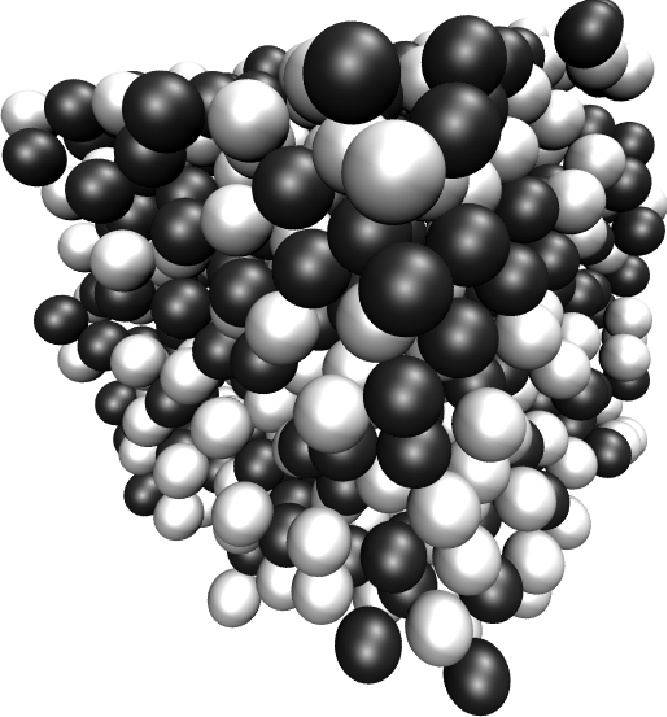
\includegraphics[width=0.4\textwidth]{figures/salt.png}
  \caption{VMD Snapshot of the salt system}
  \label{fig:snapshot}
\end{figure}

With these configurations, we can now investigate the system. As an example, we
will create a second script which calculates the averaged radial distribution
functions $g_{++}(r)$ and $g_{+-}(r)$. The radial distribution function for a
the current configuration can be obtained using the \verb|analyze| command:
\begin{tclcode}
set rdf [analyze rdf 0 1 0.9 [expr $box_l/2] 100]
set rlist ""
set rdflist ""
foreach value [lindex $rdf 1] {
  lappend rlist   [lindex $value 0]
  lappend rdflist [lindex $value 1] 
}
\end{tclcode}
The shown \verb|analyze rdf| command returns the distribution function of
particles of type 1 around particles of type 0 (i.~e.\ of opposite charges) for
radii between $0.9$ and half the box length, subdivided into $100$ bins.
Changing the first two parameters to either ``0 0'' or ``1 1'' allows to
determine the distribution for equal charges. The result is a list of $r$ and
$g(r)$ pairs, which the following foreach loop divides up onto two lists
\verb|rlist| and \verb|rdflist|.

To average over a set of configurations, we put the two last code snippets into
a loop like this:
\begin{tclcode}
set cnt 0
for {set i 0} {$i < 100} {incr i} { lappend avg_rdf 0}
foreach filename $argv {
  set f [open $filename "r"]
  while { [blockfile $f read auto] != "eof" } {}
  close $f
  set rdf [analyze rdf 0 1 0.9 [expr $box_l/2] 100]
  set rlist ""
  set rdflist ""
  foreach value [lindex $rdf 1] {
     lappend rlist   [lindex $value 0]
     lappend rdflist [lindex $value 1] }
  set avg_rdf [vecadd $avg_rdf $rdflist]
  incr cnt 
}
set avg_rdf [vecscale [expr 1.0/$cnt] $avg_rdf]
\end{tclcode}
Initially, the sum of all $g(r)$, which is stored in \verb|avg_rdf|, is set to
0.  Then the loops over all configurations given by \verb|argv|, calculates
$g(r)$ for each configuration and adds up all the $g(r)$ in \verb|avg_rdf|.
Finally, this sum is normalized by dividing by the number of
configurations. Note the ``1.0/\$cnt''; this is necessary, since ``1/\$cnt'' is
interpreted as an integer division, which results in 0 for $\text{cnt}>1$.
\verb|argv| is a predefined variable: it contains all the command line
parameters. Therefore this script should be called like
\begin{code}
Espresso \var{script} [\var{config}... ]
\end{code}

\begin{figure}[tb]
  \centering
  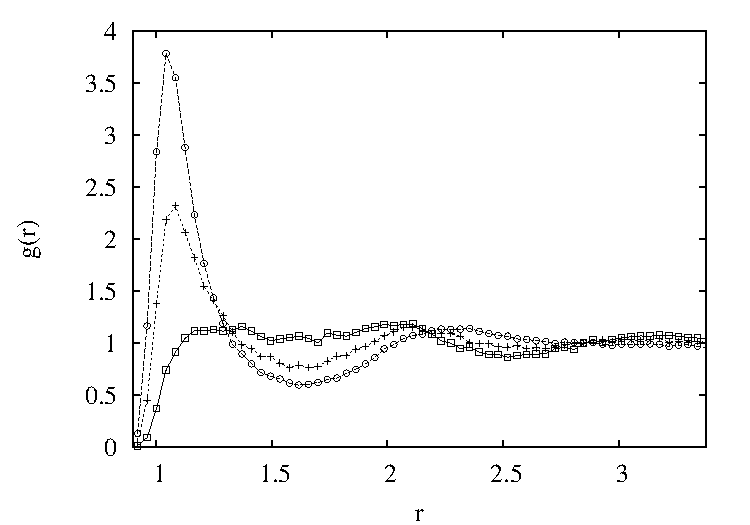
\includegraphics[width=0.7\textwidth]{figures/nacl-rdf.pdf}
  \caption{Radial distribution functions $g_{++}(r)$ between equal charges
    (rectangles) and $g_{+-}(r)$ for opposite charges (circles). The plus
    symbols denote $g(r)$ for an uncharged system.}
  \label{fig:rdf}
\end{figure}

The printing of the calculated radial distribution functions is simple. Add to the end of the
previous snippet the following lines:
\begin{tclcode}
set plot [open "rdf.data" "w"]
puts $plot "\# r rdf(r)"
foreach r $rlist rdf $avg_rdf { puts $plot "$r $rdf" }
close $plot
\end{tclcode}
This instructs the Tcl interpreter to write the \verb|avg_rdf| to the file \verb|rdf.data| in
gnuplot--compatible format. Fig.~\ref{fig:rdf} shows the resulting radial distribution functions,
averaged over 100 configurations. In addition, the distribution for a neutral
system is given, which can be obtained from our simulation script by simply
removing the command \verb|inter coulomb ...| and therefore not turning on P$^3$M.

The code example given before is still quite simple, and the reader is
encouraged to try to extend the example a little bit, e.~g. by using differently
sized particle, or changing the interactions. If something does not work, \es\
will give comprehensive error messages, which should make it easy to identify
mistakes. For real simulations, the simulation scripts can extend over thousands
of lines of code and contain automated adaption of parameters or online
analysis, up to automatic generation of data plots.  Parameters can be changed
arbitrarily during the simulation process, as needed for e.~g.\ simulated
annealing. The possibility to perform non--standard simulations without the need
of modifications to the simulation core was one of the main reasons why we
decided to use a script language for controlling the simulation core.

\section{\texttt{tutorial.tcl}}

In the directory \texttt{samples/} of the es{} sources, you will find
a well documented simulation script \texttt{tutorial.tcl}, which takes
you step by step through a slightly more complicated simulation of a
polyelectrolyte system. The basic structure of the script is however
the same as in the previous example and probably the same as the
structure of most \es{} simulation scripts.

Initially, some parameters and global variables are set, the
interactions are initialized, and particles are added. For this, the
script makes use of the \verb|polymer| command, which provides a
faster way to set up chain molecules.

The actual simulation falls apart again into two loops, the warmup
loop with increasing force capping, and the final simulation loop.
Note that the electrostatic interaction is only activated after
equilibrating the excluded volume interactions, which speeds up the
warmup phase. However, depending on the problem, this splitted warmup
may not be possible due to physical restrictions. \es{} cannot detect
these mistakes and it is your responsibility to find simulation
procedure suitable to your specific problem.

%%% Local Variables: 
%%% mode: latex
%%% TeX-master: "ug"
%%% End: 

\chapter{Compiling and installing \es}
\label{chap:install}
\index{Installation|textbf}

\begin{itemize}
\item Compiling \es{} is a necessary evil
\item Features can be compiled in or not
\item For maximal efficiency, compile in only the features that you
  use
\item \es{} can be obtained from the \es{} home page
  \footnote{\url{http://www.espresso.mpg.de}}.
\item If you are looking for the \es binary or the object files, read
  \vref{sec:builddir}
\item other than in most packages, \es will probably not be installed,
  or it will only be installed locally. Refer to \vref{sec:installdir}
  for details.
\end{itemize}

\section{Source and build directories}
\label{sec:builddir}
\index{build directory} \index{source directory}

Usually, when a program is compiled, the resulting binary files are
put into the same directory as the sources of the program. In \es, the
\emph{source directory} that contains all the source files is
completely separated from the \emph{build directory} where the files
created by the build process are put. As the source directory is not
modified during the compilation process, it is possible to compile more
than one binary versions of \es from a single set of source files.

The location of the build directory is determined when
\texttt{configure} is called.  Depending on whether it is called from
the source directory where it resides, or from some other directory,
the build system will act different.

When \texttt{configure} is called from another current working
directory than the source directory, this directory will become the
\emph{build directory}.  All files will be generated below the build
directory.  This way, you can make as many builds of \es as you like,
each build having different compiler flags and built-in features, and
for as many platforms as you want.  All further commands concerning
compiling and running \es{} have to be called from this directory,
instead of from the source directory.

When \texttt{configure} is called from the source directory where the
script resides, the \es build system has limited built-in capabilities
to handle different computer hardware.  A new subdirectory is created
in the source directory and \texttt{configure} is recursively called
from this directory, making the subdirectory the build directory.  The
directory is called \texttt{obj-}\textit{platform}\texttt{/}, where
\textit{platform} is an automatically determined descriptor of the CPU
type where the script was started, \eg
\mbox{\texttt{obj-Athlon\_64-pc-linux}}.  Note that this heuristic
will work in many cases, but it may not always work as intended.  When
you notice any problems, you can always call \texttt{configure} from
another directory.

In this case it is also possible to run the commands \texttt{make} and
\texttt{Espresso} directly in the source directory.  Furthermore, the
option \texttt{--enable-chooser} will be set in the recursive call of
\texttt{configure} that activates the automatic binary chooser (see
section \vref{sec:installdir}).

\paragraph{Example}
When the source directory is \texttt{\$srcdir} (\ie{} the files where
unpacked to this directory), then the build directory can be set to
\texttt{\$builddir} by calling the \texttt{configure}-script from
there:
\begin{code}
cd $builddir
$srcdir/configure
make
Espresso
\end{code}

\section{\texttt{myconfig.h}: Activating and deactivating features}
\label{sec:myconfig}

\index{features} \index{myconfig.h} \index{configuration header} \es
has a large number of features that can be compiled into the binary.
However, it is not recommended to actually compile in all possible
features, as this will negatively affect \es's performance.  Instead,
compile in only the features that are actually required.  For the
developers, it is also possible to turn on or off a number of
debugging messages.  The features and debug messages can be controlled
via a configuration header file that contains C-preprocessor
declarations. Appendix \vref{chap:features} lists and describes all
available features.  When no configuration header is provided by the
user, a default header will be used that turns on the default
features.  The file \texttt{myconfig-sample.h} in the source directory
contains a list of all possible features that can be copied into your
own configuration file.

When you distinguish between the build and the source directory (see
\vref{sec:builddir}), the configuration header can be put in either of
these. Note, however, that when a configuration header is found in
both directories, the one in the build directory will be used.  For an
example how this can be employed, see section \ref{sec:builddir}.

By default, the configuration header is called \texttt{myconfig.h}.
The name of the configuration header can be changed either when the
\texttt{configure}-script is called with the option
\mbox{\texttt{--with-myconfig}} (see section \vref{sec:configure}), or
when \texttt{make} is called with the setting
\mbox{\texttt{myconfig=}\textit{myconfig\_header}} (see section
\vref{sec:make}).

The configuration header can be used to compile different binary
versions of \es with a different set of features from the same source
directory.  Suppose that you have a source directory \texttt{\$srcdir}
and two build directories \texttt{\$builddir1} and
\texttt{\$builddir2} that contain different configuration headers:

\begin{itemize}
\item \texttt{\$builddir1/myconfig.h}:
\begin{code}
#define ELECTROSTATICS
#define LENNARD-JONES
\end{code}

\item \texttt{\$builddir2/myconfig.h}:
\begin{code}
#define LJCOS
\end{code}
\end{itemize}

\noindent Then you can simply compile two different versions of \es via
\begin{code}
cd $builddir1
$srcdir/configure
make

cd $builddir2
$srcdir/configure
make
\end{code}


\section{Running \texttt{configure}}
\label{sec:configure}

% Description of basic options: --prefix, --exec-prefix, CPPFLAGS,
% CFLAGS, LDFLAGS

\index{configure} The shell script \texttt{configure} collects all the
information required by the compilation process. It will determine how
to use and where to find the different libraries and tools required by
the compilation process, and it will test what compiler flags are to
be used.  The script will find out most of these things automatically.
If something is missing, it will complain and give hints how to solve
the problem.  The generic syntax of calling the \texttt{configure}
script is:
\begin{code}
configure [\var{options} ...] [\var{variable}=\var{value} ...]
\end{code}

\noindent Note that in the \es build system, the files generated by
the configuration and compilation process are not placed next to the
source files, but into a separate \emph{build directory} instead.
Refer to section \vref{sec:builddir} for details.

\index{configure options} The behaviour of \texttt{configure} can be
controlled by the means of command line options. In the following,
only those command line options that are specific to \es will be
explained.  For a complete list of options and explanations thereof,
call
\begin{code}
configure --help
\end{code}

\subsection{Options}

\begin{description}
\item [\texttt{--enable-chooser}] This option will enable the
  automatic binary chooser mechanism for \es (see section
  \vref{sec:installdir}).  This option will be automatically enabled,
  when the \texttt{configure} script is called from the source
  directory, otherwise it will be disabled. It is not recommended to
  set the option manually.
\item[\texttt{--enable-debug}] This option will enable compiler flags
  required for debugging the \es binary and is disabled by default.
\item[\texttt{--enable-profiling}] This option will enable compiler
  flags required for profiling the \es binary and is disabled by
  default.
\item[\texttt{--disable-processor-optimization}] This option will
  control whether \texttt{configure} will check for several
  optimization flags to be used by the compiler. This option is
  enabled by default.
\item[\texttt{--disable-xlc-qipa}] This option is only useful when the
  IBM C-compiler \texttt{xlc} is used and will control whether or not
  the compiler flag \texttt{-qipa} is used.  If you come upon problems
  when using the \es binary on IBM machines, try using
  \texttt{--disable-xlc-ipa}. The option is enabled by default.
\item[\texttt{--with-myconfig=MYCONFIG\_HEADER}] This option sets the
  name of the local configuration header (see \vref{sec:myconfig}). It
  defaults to ``\texttt{myconfig.h}''.
\item[\texttt{--with-mpi=MPI}/ \texttt{--without-mpi}] Sets the MPI
  implementation that should be used, or disables MPI. By default,
  \texttt{configure} will test automatically what MPI implementation
  is available. The following implementations are known:
  \begin{description}
  \item[\texttt{fake}, \texttt{no}] This will disable MPI
    completely. Equivalent to \mbox{\texttt{--without-mpi}}.
  \item[\texttt{lam}] Use the LAM/MPI environment
    (\url{http://www.lam-mpi.org/}).
  \item[\texttt{mpich}] Use the MPICH environment
    (\url{http://www-unix.mcs.anl.gov/mpi/mpich/}).
  \item[\texttt{poe}] Use the POE environment (IBM).
  \item[\texttt{dmpi}] Use the DMPI environment (Tru64).
  \item[\texttt{generic}] Use a generic MPI implementation. This will
    try to find an MPI compiler and an MPI runtime environment.
  \end{description}
\item[\texttt{--with-efence} / \texttt{--without-efence}] Whether or
  not to use the ``electric fence'' memory debugging library
  (\url{http://freshmeat.net/projects/efence/}). Efence is not used by
  default.
\item[\texttt{--with-tcl=TCL}] By default, \texttt{configure} will
  automatically determine which version of Tcl is used.  If the wrong
  version is chosen automatically, you can specify the name of the
  library with this option, \eg{} \texttt{tcl8.4}.
\item[\texttt{--with-tk=TK} / \texttt{--without-tk}] By default, the
  GUI toolkit Tk is not used by \es. This option can be used to
  activate Tk and to specify which Tk version to use, \eg{}
  \texttt{tk8.4}. If you only specify \texttt{--with-tk} and do not
  give a version number, \texttt{configure} will try to automatically
  deduce the right version.
\item[\texttt{--with-fftw=VERSION} / \texttt{--without-fftw}] This can
  be used to specify whether the FFTW library is to be used, and which
  version.  By default, version 3 will be used if it is found,
  otherwise version 2 is used.  Note that quite a number of central
  features of \es require FFTW.
\end{description}

\section{\texttt{make}: Compiling,  testing and installing \es}
\label{sec:make}

The command \texttt{make} is mainly used to compile the \es{} source
code, but it can do a number of other things. The generic syntax of
the \texttt{make} command is:
\begin{code}
make [\var{target}...] [\var{variable}=\var{value}]
\end{code}
When no target is given, the target \texttt{all} is used. The
following targets are available:
\begin{description}
\item[\texttt{all}] Compiles the complete \es source code. The
  variable \lit{myconf} can be used to specify the name of the
  configuration header to be used.
\item[\texttt{check}] Runs the testsuite. By default, all available
  tests will be run on 1, 2, 3, 4, 6, or 8 processors. Which tests are
  run can be controlled by means of the variable \texttt{tests}, which
  processor numbers are to be used can be controlled via the variable
  \texttt{processors}. Note that depending on your MPI installation,
  MPI jobs can only be run in the queueing system, so that \es{} will
  not run from the command line. In that case, you may not be able to
  run the testsuite, or you have to directly submit the testsuite script
  \verb!testsuite/test.sh! to the queueing system.\\
  \textbf{Example:} \verb!make check tests="madelung.tcl" processors="1 2"!\\
  will run the test \texttt{madlung.tcl} on one and two processors.
\item[\texttt{clean}] Deletes all files that were created during the
  compilation.
\item[\texttt{mostlyclean}] Deletes most files that were created
  during the compilation. Will keep for example the built doxygen
  documentation and the \es{} binary.
\item[\texttt{dist}] Creates a \texttt{.tar.gz}-file of the \es{}
  sources.  This will include all source files as they currently are
  in the source directory, \ie{} it will include local changes.  This
  is useful to give your version of \es{} to other people.
  The variable \texttt{extra} can be used to specify additional
  files and directories that are to be included in the archive
  file. \\
  \textbf{Example:} \verb!make dist extra="myconfig.h internal"!\\
  will create the archive file and include the file
  \texttt{myconfig.h} and the directory \texttt{internal} with all
  files and subdirectories.
\item[\texttt{install}] Install \es. The variables \texttt{prefix} and
  \texttt{exec-prefix} can be used to specify the installation
  directories, otherwise the defaults defined by the
  \texttt{configure} script are used. \texttt{prefix} sets the prefix
  where all \es files are to be installed, \texttt{exec-prefix} sets
  the prefix where the executable files are to be installed and is
  required only when there is an architecture-specific directory (\eg
  \texttt{/usr/local/bin64/}).  For the actual locations where the
  different files are installed, refer to section
  \vref{sec:installdir}.\\
  \textbf{Example:} \verb!make install prefix=/usr/local!\\
  will install all files below \texttt{/usr/local}.
\item[\texttt{uninstall}] Uninstalls \es{}, \ie{} removes all files
  that were installed during \texttt{make install}. The variables are
  identical to the variables of the \texttt{install}-target.
\end{description}

\subsection{Installation directories}
\label{sec:installdir}

\index{installation directory} Other than most software, \es is not
necessarily installed into the system, but can also be used directly
from the build directory.  The rest of this section is only
interesting if you plan to install \es.

Normally, the \es-binary \texttt{Espresso-bin} is installed in the
directory \texttt{\$prefix/libexec/} and a the wrapper script
\texttt{Espresso} in the directory \texttt{\$prefix/bin/} that handles
the MPI invocation.

When the \texttt{configure}-script is called from the source directory
or when the option \texttt{--enable-chooser} is given, an automatic
binary chooser is installed in the directory \texttt{\$prefix/bin/}
and the \es-binary and the MPI wrapper script are installed in an
architecture-specific subdirectory
\mbox{\texttt{\$exec-prefix/lib/espresso/obj-}\textit{platform}\texttt{/}}.
When called, the binary chooser will automatically call the MPI
wrapper script from the right subdirectory.

\section{Running \es}
\label{sec:run}

When \es is found in your path, it can be run via
\begin{code}
Espresso [\var{tcl\_script} [\var{N\_processors} [\var{args}]]]
\end{code}

\index{interactive mode} When \es{} is called without any arguments,
it is started in the interactive mode, where new commands can be
entered on the command line. When the name of a \textit{tcl\_script}
is given, the script is executed. \textit{N\_processors} is the number
of processors that are to be used. Any further arguments are passed to
the script. Note that depending on your MPI installation, MPI jobs can
only be run in the queueing system, so that \es will not run from
the command line.

% A number of wrapper scripts are used in running \es{}:
% \begin{itemize}
% \item The script \texttt{Espresso} in the source and build directory
%   will try to run the compiled version of \es. If it is called from
%   the source directory, it assumes that \es{} was also configured in
%   the source directory and will try to recursively start the script in
%   the corresponding \texttt{obj-PLATFORM} build directory. If it is
%   called in the build directory, it will start the \es-binary with the
%   right MPI implementation.
% \item The chooser script \texttt{Espresso} 
%   \begin{itemize}
%   \item installed when \verb!--enable-chooser! was given
%   \item installed to bindir
%   \item tries to run the correct version of the MPI-wrapper
%     \texttt{Espresso}
%   \end{itemize}
% \item The MPI-wrapper \texttt{Espresso}
%   \begin{itemize}
%   \item installed next to \es{} binary
%   \item starts the binary with the right MPI implementation
%   \end{itemize}
% \item The \es{} binary \texttt{Espresso-bin} can also be started
%   directly, however, it requires that the environment variable
%   \verb!ESPRESSO_SCRIPTS! is set to the directory where the scripts
%   are installed (usually \verb!$(prefix)/lib/espresso/scripts! or
%   \verb!$(prefix)/share/espresso/scripts!).
% \end{itemize}


%%% Local Variables: 
%%% mode: latex
%%% TeX-master: "ug"
%%% End: 

\chapter{Setting up the system}
\label{chap:setup}

\section{\texttt{setmd}: Setting global variables.}
\newescommand{setmd}

\begin{essyntax}
\variant{1} setmd \var{variable}
\variant{2} setmd \var{variable} \opt{\var{value}}+
\end{essyntax}
\todo{Explain '+' in intro.}

Variant \variant{1} returns the value of the \es global variable
\var{variable}, variant \variant{2} can be used to set the variable
\var{variable} to \var{value}. The following global variables can be
set:

%% List-environment for the description of the global variables
\newenvironment{globvar}{
  \begin{list}{}{
      \setlength{\rightmargin}{1em}
      \setlength{\leftmargin}{2em}
      \setlength{\partopsep}{0pt}
      \setlength{\topsep}{1ex}
      \setlength{\parsep}{0.5ex}
      \setlength{\listparindent}{-1em}
      \setlength{\labelwidth}{0.5em}
      \setlength{\labelsep}{0.5em}
      \renewcommand{\makelabel}[1]{%
        \index{##1@\texttt{##1} (global variable)|mainindex}%
        \index{global variables!\texttt{##1}|mainindex}%
        \texttt{##1}%
      }
    }
  }{
  \end{list}
}
\newcommand{\ro}{\emph{read-only}}

\todo{Better throw some out (\eg switches)?}
\todo{Missing: lattice_switch, dpd_tgamma, n_rigidbonds}
\todo{Which commands can be used to set the \emph{read-only}
  variables?}
\begin{globvar}
\item[box_l] (double[3]) Simulation box length.
  \todo{document what happens to the particles when \keyword{box_l} is
    changed!}
\item[cell_grid] (int[3], \ro) Dimension of the inner
  cell grid.
\item[cell_size] (double[3], \ro) Box-length of a cell.
\item[dpd_gamma] (double, \ro) Friction constant for the
  DPD thermostat.
\item[dpd_r_cut] (double, \ro) Cutoff for DPD thermostat.
\item[gamma] (double, \ro) Friction constant for the
  Langevin thermostat.
\item[integ_switch] (int, \ro) Internal switch which integrator to
  use.
\item[local_box_l] (int[3], \ro) Local simulation box length of the
  nodes.
\item[max_cut] (double, \ro) Maximal cutoff of real space
  interactions.
\item[max_num_cells] (int) Maximal number of cells for the link cell
  algorithm.  Reasonable values are between 125 and 1000, or for some
  problems (\var{n_total_particles} / \var{n_nodes}).
\item[max_part] (int, \ro) Maximal identity of a particle.
  \emph{This is in general not related to the number of particles!}
\item[max_range] (double, \ro) Maximal range of real space
  interactions: \var{max_cut} + \var{skin}.
\item[max_skin] (double, \ro) Maximal skin to be used for the link
  cell/verlet algorithm. This is the minimum of \var{cell_size} -
  \var{max_range}. \todo{???}
\item[min_num_cells] (int) \todo{???} Minimal number of cells for the
  link cell algorithm. Reasonable values range in $1e-6 N^2$ to $1e-7
  N^2$. In general just make sure that the Verlet lists are not
  incredibly large. By default the minimum is 0, but for the automatic
  P3M tuning it may be wise to larger values for high particle
  numbers.
\item[n_layers] (int, \ro) Number of layers in cell structure LAYERED
  (see section \vref{sec:cell-systems}).
\item[n_nodes] (int, \ro) Number of nodes.
\item[n_part] (int, \ro) Total number of particles.
\item[n_part_types] (int, \ro) Number of particle types that were
  used so far in the \keyword{inter} command (see chapter{tcl:inter}).
\item[node_grid] (int[3]) 3D node grid for real space domain
  decomposition (optional, if unset an optimal set is chosen
  automatically).
\item[nptiso_gamma0] (double, \ro)\todo{Docs missing.}
\item[nptiso_gammav] (double, \ro)\todo{Docs missing.}
\item[npt_p_ext] (double, \ro) Pressure for NPT simulations.
\item[npt_p_inst] (double) Pressure calculated during an
  NPT_isotropic integration.
\item[piston] (double, \ro) Mass off the box when using NPT_isotropic
  integrator.
\item[periodicity] (bool[3]) Specifies periodicity for the three
  directions. If the feature PARTIAL_PERIODIC is set, this variable
  can be set to (1,1,1) or (0,0,0) at the moment.  If not it is
  readonly and gives the default setting (1,1,1).\todo{Correct?}
\item[skin] (double) Skin for the Verlet list.
\item [temperature] (double, \ro) Temperature of the
  simulation.
\item[thermo_switch] (double, \ro) Internal variable which thermostat
  to use. 
\item[time] (double) The simulation time.
\item[time_step] (double) Time step for MD integration.
\item[timings] (int) Number of timing samples to take into account if
  set.\todo{???}
\item[transfer_rate] (int, \ro) Transfer rate for VMD connection. You
  can use this to transfer any integer value to the simulation from
  VMD.
\item[verlet_flag] (bool) Indicates whether the Verlet list will be
  rebuild. The program decides this normally automatically based on
  your actions on the data.
\item[verlet_reuse] (double) Average number of integration steps the
  verlet list has been re-used.
\end{globvar}

\section{\texttt{thermostat}: Setting up the thermostat}
\newescommand{thermostat}

\begin{essyntax}
  \variant{1} thermostat off
  \variant{2} theormstat \var{method} \opt{\var{parameter}}+
\end{essyntax}
\todo{Include docs from \texttt{thermostat.h}!}
Change thermostat settings.

\section{\texttt{nemd}: Setting up non-equilibrium MD}
\newescommand{nemd}

\begin{essyntax}
  \variant{1}nemd \var{method} \var{parameter} 
  \variant{2}nemd off
  \variant{3}nemd profile
  \variant{4}nemd viscosity
\end{essyntax}
\todo{Include docs from \texttt{nemd.h}!}
\todo{Put \texttt{nemd profile|viscosity} into \texttt{analyze}?}  
Use NEMD (Non Equilibrium Molecular Dynamics) to simulate a system
under shear.

\section{\texttt{cellsystem}: Setting up the cell system}
\label{sec:cell-systems}
\newescommand{cellsystem}

This section deals with the flexible particle data organization of
\es.  Due to different needs of different algorithms, \es is able to
change the organization of the particles in the computer memory,
according to the needs of the used algorithms. For details on the
internal organization, refer to section
\vref{sec:internal-particle-organization}.

\subsection{Domain decomposition}
\index{domain decomposition}
\begin{essyntax}
  cellsystem domain_decomposition \opt{-no_verlet_list}
\end{essyntax}
This selects the domain decomposition cell scheme, using Verlet lists
for the calculation of the interactions. If you specify
\keyword{-no_verlet_list}, only the domain decomposition is used, but
not the Verlet lists.

The domain decomposition cellsystem is the default system and suits
most applications with short ranged interactions. The particles are
divided up spatially into small compartments, the cells, such that the
cell size is larger than the maximal interaction range. In this case
interactions only occur between particles in adjacent cells. Since the
interaction range should be much smaller than the total system size,
leaving out all interactions between non-adjacent cells can mean a
tremendous speed-up. Moreover, since for constant interaction range,
the number of particles in a cell depends only on the density. The
number of interactions is therefore of the order N instead of order
$N^2$ if one has to calculate all pair interactions.

\subsection{N-squared}
\begin{essyntax}
  cellsystem nsquare 
\end{essyntax}
This selects the very primitive nsquared cellsystem, which calculates
the interactions for all particle pairs. Therefore it loops over all
particles, giving an unfavorable computation time scaling of $N^2$.
However, algorithms like MMM1D or the plain Coulomb interaction in the
cell model require the calculation of all pair interactions.

In a multiple processor environment, the nsquared cellsystem uses a
simple particle balancing scheme to have a nearly equal number of
particles per CPU, \ie $n$ nodes have $m$ particles, and $p-n$ nodes
have $m+1$ particles, such that $n*m+(p-n)*(m+1)=N$, the total number
of particles. Therefore the computational load should be balanced
fairly equal among the nodes, with one exception: This code always
uses one CPU for the interaction between two different nodes. For an
odd number of nodes, this is fine, because the total number of
interactions to calculate is a multiple of the number of nodes, but
for an even number of nodes, for each of the $p-1$ communication
rounds, one processor is idle.

E.g. for 2 processors, there are 3 interactions: 0-0, 1-1, 0-1.
Naturally, 0-0 and 1-1 are treated by processor 0 and 1, respectively.
But the 0-1 interaction is treated by node 1 alone, so the workload
for this node is twice as high. For 3 processors, the interactions are
0-0, 1-1, 2-2, 0-1, 1-2, 0-2. Of these interactions, node 0 treats 0-0
and 0-2, node 1 treats 1-1 and 0-1, and node 2 treats 2-2 and 1-2.

Therefore it is highly recommended that you use nsquared only with an
odd number of nodes, if with multiple processors at all. 

\subsection{Layered cell system}
\begin{essyntax}
  cellsystem layered \var{n_layers}
\end{essyntax}

This selects the layered cell system, which is specifically designed
for the needs of the MMM2D algorithm. Basically it consists of a
nsquared algorithm in x and y, but a domain decomposition along z, i.
e. the system is cut into equally sized layers along the z axis. The
current implementation allows for the cpus to align only along the z
axis, therefore the processor grid has to have the form 1x1xN.
However, each processor may be responsible for several layers, which
is determined by \var{n\_layers}, i. e. the system is split into
N*\var{n\_layers} layers along the z axis. Since in x and y direction
there are no processor boundaries, the implementation is basically
just a stripped down version of the domain decomposition cellsystem.

%%% Local Variables: 
%%% mode: latex
%%% TeX-master: "ug"
%%% End: 

\chapter{Running the simulation}
\label{chap:run}

\section{\texttt{integrate}: Running the simulation}
\eslabel{integrate}

\begin{essyntax}
  \variant{1} integrate \var{steps}
  \variant{2} integrate set \var{method} \opt{\var{parameter}}+
\end{essyntax}

\todo{Docs missing!}
\todo{Which integrators do exist?}

\section{\texttt{change_volume}: Changing the box volume}
\eslabel[change-volume]{change_volume}

\begin{essyntax}
  \variant{1} change_volume \var{V_new} 
  \variant{2} change_volume \var{L_new} \alt{x \asep y \asep z \asep xyz}
\end{essyntax}
Changes the volume of either a cubic simulation box to the new volume
\var{V_new} or its given x-/y-/z-/xyz-extension to the new box-length
\var{L_new}, and isotropically adjusts the particles coordinates as
well. The function returns the new volume of the deformed simulation
box.

\section{Stopping particles}
\eslabel{stopParticles}
\eslabel[stop-particles]{stop_particles}

\begin{essyntax}
  \variant{1} stopParticles
  \variant{2} stop_particles
\end{essyntax}
Halts all particles in the current simulation, setting their
velocities and forces to zero. Variant \variant{2} does not provide
feedback on the execution status.

\section{\texttt{velocities}: Setting the velocities}
\eslabel{velocities}
\begin{essyntax}
  velocities \var{v_max} 
  \opt{start \var{part_id}} 
  \opt{count \var{N_T}}
\end{essyntax}
Sets the velocities of the particles with particle ID (see The part
command) between \var{part_id} and \var{part_id}+\var{N_T}
(defaults to '0' \& '[setmd npart]-\var{part_id}') to a random vector
with length in [-vmax,vmax], and returns the absolute value of the
total velocity assigned.

\section{\texttt{invalidate_system}}
\eslabel[invalidate-system]{invalidate_system}
\begin{essyntax}
  invalidate_system
\end{essyntax}
\todo{Documentation not up to date!}

Forces a system re-init which, among others, causes the integrator to
also update the forces at its beginning (instead of re-using the
values from the previous integration step).  This is particularly
necessary to ensure continuity after setting a checkpoint:
\texttt{integrate} - \texttt{set_checkpoint} - \texttt{integrate} has
only one call to \todo{???}???, while \texttt{read_checkpoint} -
\texttt{integrate} has two at the beginning of the 2nd integrate
(because loading a new system from disk typically requires
re-initializing the system), and since ??? also uses the thermostat
which in turn draws random numbers, the two situations do not end up
at the same segment of the random number sequence, all random events
will therefore slightly differ.  To prevent this, simply include a
call to invalidate_system upon setting the checkpoint (this is being
done automatically if using tcl_checkpoint_set and
tcl_checkpoint_read beginning with v1.1 of \es{}), because in that
case both scenarios will call ??? twice at the beginning of the second
integration phase thus having their random number sequences in total
sync. The C implementation is invalidate_system.



%%% Local Variables: 
%%% mode: latex
%%% TeX-master: "ug"
%%% End: 

\chapter{Analysis}
\label{chap:analysis}


%%% Local Variables: 
%%% mode: latex
%%% TeX-master: "ug"
%%% End: 

\chapter{Auxilliary commands}
\label{chap:aux}

\section{Writing VTF files}
%\quickrefheading{Handling of VTF files}

There are two commands in \es{} that support writing files in the VMD
formats VTF, VSF and VCF.\footnote{A description of the format and a
  plugin to read the format in VMD is found in the subdirectory
  \texttt{vmdplugin/} of the \es{} source directory.} The commands can
be used to write the structure (\texttt{writevsf}) and coordinates
(\texttt{writevcf}) of the system to a single trajectory file (usually
with the extension \texttt{.vtf}), or to separate files (extensions
\texttt{.vsf} and \texttt{.vtf}).

\subsection{\texttt{writevsf}}

\tclcommand{writevsf}
{\var{file} [<short|verbose>] [<\var{radii}|auto>] [typedesc \var{typedesc}]}

Writes a structure block describing the system's structure to
\var{file}. The atom ids used in the file are identical to \es's
particle ids.  This makes it easy to write additional structure lines
to the file, e.g. to specify the \texttt{resname} of particle
compounds, like chains.  The output of this file can be used in a
standalone VSF file, or at the beginning of a trajectory VTF file that
contains a trajectory of a whole simulation.

\begin{tcloptions}
  \option{<short|verbose>}
  Specify, whether the output is in a human-readable, but somewhat
  longer format (\keyword{verbose}), or in a more compact form
  (\keyword{short}). The default is \keyword{verbose}.
  
  \option{<radius \var{radii}|auto>}
  Specify the VDW radii of the atoms. \var{radii} is either
  \keyword{auto}, or a Tcl-list describing the radii of the different
  particle types. When the keyword \keyword{auto} is used and a
  Lennard-Jones interaction between two particles of the given type is
  defined, the radius is set to be $\frac{\sigma_{LJ}}{2}$ plus the LJ
  shift.  Otherwise, the radius $0.5$ is substituted. The default is
  \keyword{auto}.
  
  Example: \verb!writevsf "show.tcl" radius {{0 2.0} {1 auto} {2 1.0}}!
  
  \option{typedesc \var{typedesc}}
  \var{typedesc} is a Tcl-list giving additional VTF atom-keywords to
  specify additional VMD characteristics of the atoms of the given type.
  If no description is given for a certain particle type, it defaults to
  \texttt{segid \textit{n}}, where \textit{n} is the type id.

  Example: \verb!writevsf "show.tcl" typedesc {{0 "segid colloid"} {1 "segid pe"}}!
\end{tcloptions}


\subsection{\texttt{writevcf}}
\tclcommand{writevcf}
{\var{file} [<short|verbose>] [<folded|absolute>]}

Writes a coordinate (or timestep) block that contains all coordinates
of the system's particles to \var{file}.

\begin{tcloptions}
  \option{<short|verbose>} Specify, whether the output is in a
  human-readable, but somewhat longer format (\keyword{verbose}), or
  in a more compact form (\keyword{short}). The default is
  \keyword{verbose}.

  \option{<folded|absolute>} Specify whether the particle positions
  are written in absolute coordinates (\keyword{absolute}) or folded
  into the central image of a periodic system (\keyword{folded}). The
  default is \keyword{absolute}.

  \option{<pids \var{pids}|all>} Specify the coordinates of which particles
  should be written. If \keyword{all} is used, all coordinates will be
  written (in the ordered timestep format). Otherwise, \var{pids} has
  to be a Tcl-list specifying the pids of the particles. The default
  is \keyword{all}.
  
  Example: \verb!pids {0 23 42}!

\end{tcloptions}


%%% Local Variables: 
%%% mode: latex
%%% TeX-master: "ug"
%%% End: 

\chapter{Under the hood}
\label{chap:underhood}

(new)

\begin{itemize}
\item Implementation issues that are interesting for the user
\item Main loop in pseudo code (for comparison)
\item from doxygen: ``Cell systems'' 
\end{itemize}

%%% Local Variables: 
%%% mode: latex
%%% TeX-master: "ug"
%%% End: 

\chapter{Getting involved}
\label{chap:devel}

\begin{itemize}
\item What to do when you want to become involved
\item How to submit a bug report
\item Reference to developer's guide
\end{itemize}

%%% Local Variables: 
%%% mode: latex
%%% TeX-master: "ug"
%%% End: 


\appendix
\chapter{\es{} quick reference}
\label{chap:quickref}

\index{quick reference of Tcl-commands}
%\input{ug.qrf}
%\listofcommands

%%% Local Variables: 
%%% mode: latex
%%% TeX-master: "ug"
%%% End: 

\chapter{Features}
\label{sec:features}
\index{features|textbf}

\newcommand{\feature}[1]{\texttt{\textbf{#1}}}

This chapter describes the features that can be activated in \es. Even
if possible, it is not recommended to activate all features, because
this will negatively effect \es's performance.

Features can be activated in the configuration header (see section
\vref{sec:myconfig}). Too activate \texttt{FEATURE}, add the following
line to the header file:
\begin{verbatim}
#define FEATURE
\end{verbatim}

\subsection{General features}
\begin{itemize}
\item \feature{PARTIAL\_PERIODIC} By default, all coordinates in \es{} are periodic. With
  \texttt{PARTIAL\_PERIODIC} turned on, the \es{} global variable \texttt{periodic} (see
  Sec.~\ref{sec:globalvar}) controls the periodicity of the individual coordinates. Note that this
  slows the integrator down by around $10-30\%$.
\item \feature{ELECTROSTATICS} This switches on the various electrostatics algorithms, such as
  the Ewald summation. See Sec.~\ref{sec:electrostatics} for details on this algorithms.
\item \feature{ROTATION} Switch on rotational degrees of freedom for the particles, as well as
  the corresponding quaternion integrator. See Sec.~\ref{sec:rotation} for details.
\item \feature{DIPOLES} This activates the dipole support in P$^3$M. Currently, a mixing of
  dipoles and charges is not possible, i.~e. all particles have to have charge $q=0$.
  Requires \texttt{ELECTROSTATICS} and \texttt{ROTATION}.
\item \feature{EXTERNAL\_FORCES} Allows to define an arbitrary constant force for each particle
  individually. Also allows to fix individual coordinates of particles, e.~g. keep them at a fixed
  position or within a plane.
\item \feature{CONSTRAINTS} Turns on various spatial constraints such as spherical compartments
  or walls. This constraints interact with the particles through regular short ranged potentials
  such as the Lennard--Jones potential. See Sec.~\ref{sec:constraints} for possible constraint
  forms.
\item \feature{MASS} Allows particles to have individual masses. Note that some analyzation
  procedures have not yet been adapted to take the masses into account correctly.
\item \feature{EXCLUSIONS} Allows to exclude specific short ranged interactions within
  molecules, which is necessary for some atomistic models.
\item \feature{COMFORCE}
\item \feature{COMFIXED}
\item \feature{MOLFORCES}
\item \feature{BOND\_CONSTRAINT} Turns on the RATTLE integrator which allows for fixed lengths
  bonds between particles.
\end{itemize}

In addition, there are switches that enable additional features in the integrator:
\begin{itemize}
\item \feature{NEMD} Enables the non-equilbrium (shear) MD support (see Sec.~\ref{sec:NEMD}).
\item \feature{NPT} Enables an on--the--fly NPT integration scheme (see Sec.~\ref{sec:NPT}).
\item \feature{DPD} Enables the dissipative particle dynamics thermostat (see
  Sec.~\ref{sec:DPD}).
\item \feature{LB} Enables the lattice-Boltzmann fluid code (see Sec.~\ref{sec:LB}).
\end{itemize}

\subsection{Interactions}
The following switches turn on various short ranged interactions (see Sec.~\ref{sec:shortrange}):
\begin{itemize}
\item \feature{TABULATED} Enable support for user--defined interactions, e.~g. for atomistic
  simulations.
\item \feature{LENNARD\_JONES} Enable the Lennard--Jones potential.
\item \feature{LJ\_WARN\_WHEN\_CLOSE} This adds an additional check to the Lennard--Jones
  potential that prints a warning of particles come too close so that the simulation becomes
  unphysical.
\item \feature{MORSE} Enable the Morse potential.
\item \feature{LJCOS} Enable the Lennard--Jones potential with a cosine--tail.
\item \feature{LJCOS2}
\item \feature{BUCKINGHAM} Enable the Buckingham potential.
\item \feature{SOFT\_SPHERE} Enable the soft sphere potential.
\end{itemize}

If you want to use angle bonds, you currently need to choose the type
a priori (see section \vref{sec:angle}). This will change in the near
future to three independent angle potentials:
\begin{itemize}
\item \feature{BOND\_ANGLE\_HARMONIC}
\item \feature{BOND\_ANGLE\_COSINE}
\item \feature{BOND\_ANGLE\_COSSQUARE}
\end{itemize}

\subsection{Debug messages}
Finally, there are a number of flags for debugging. The most important one are
\begin{itemize}
\item \feature{ADDITIONAL\_CHECKS} Enables numerous additional checks which can detect
  inconsistencies especially in the cell systems. This checks are however too slow to be enabled in
  production runs.
\item \feature{MEM\_DEBUG} Enables an internal memory allocation checking system. This produces
  output for each allocation and freeing of a memory chunk, and therefore allows to track down
  memory leaks. This works by internally replacing \texttt{malloc}, \texttt{realloc} and
  \texttt{free}.
\end{itemize}

The following flags control the debug output of various sections of Espresso. You will however
understand the output very often only by looking directly at the code.
\begin{itemize}
\item \feature{COMM\_DEBUG} Output from the asynchronous communication code.
\item \feature{EVENT\_DEBUG} Notifications for event calls, i.~e. the \texttt{on\_?} functions
  in \texttt{initialize.c}. Useful if some module does not correctly respond to changes of e.~g.
  global variables.
\item \feature{INTEG\_DEBUG} Integrator output.
\item \feature{CELL\_DEBUG} Cellsystem output.
\item \feature{GHOST\_DEBUG} Cellsystem output specific to the handling of ghost cells and the
  ghost cell communication.
\item \feature{GHOST\_FORCE\_DEBUG}
\item \feature{VERLET\_DEBUG} Debugging of the Verlet list code of the domain decomposition cell
  system.
\item \feature{LATTICE\_DEBUG} Universal lattice structure debugging.
\item \feature{HALO\_DEBUG}
\item \feature{GRID\_DEBUG}
\item \feature{PARTICLE\_DEBUG} Output from the particle handling code.
\item \feature{P3M\_DEBUG}
\item \feature{ESR\_DEBUG} debugging of P$^3$Ms real space part.
\item \feature{ESK\_DEBUG} debugging of P$^3$Ms $k$--space part.
\item \feature{EWALD\_DEBUG}
\item \feature{FFT\_DEBUG} Output from the unified FFT code.
\item \feature{MAGGS\_DEBUG}
\item \feature{RANDOM\_DEBUG}
\item \feature{FORCE\_DEBUG} Output from the force calculation loops.
\item \feature{THERMO\_DEBUG} Output from the thermostats.
\item \feature{LJ\_DEBUG} Output from the Lennard--Jones code.
\item \feature{MORSE\_DEBUG} Output from the Morse code.
\item \feature{FENE\_DEBUG}
\item \feature{ONEPART\_DEBUG} Define to a number of a particle to obtain output on the forces
  calculated for this particle.
\item \feature{STAT\_DEBUG}
\item \feature{POLY\_DEBUG}
\item \feature{MOLFORCES\_DEBUG}
\item \feature{LB\_DEBUG} Output from the lattice--Boltzmann code.
\item \feature{ASYNC\_BARRIER} Introduce a barrier after each asynchronous command
  completion. Helps in detection of mismatching communication.
\item \feature{FORCE\_CORE} Causes \es{} to try to provoke a core dump when exiting
  unexpectedly.
\item \feature{MPI\_CORE} Causes \es{} to try this even with MPI errors.
\end{itemize}

%%% Local Variables: 
%%% mode: latex
%%% TeX-master: "ug"
%%% End: 


\chapter{The MMM family of algorithms}
\label{chap:mmm}

\chapter{Maggs algorithm}
\label{chap:maggs}

\printindex

\end{document}


%%% Local Variables: 
%%% mode: latex
%%% TeX-master: t
%%% End: 

%\listofcommands

%%% Local Variables: 
%%% mode: latex
%%% TeX-master: "ug"
%%% End: 

\chapter{Features}
\label{sec:features}
\index{features|textbf}

\newcommand{\feature}[1]{\texttt{\textbf{#1}}}

This chapter describes the features that can be activated in \es. Even
if possible, it is not recommended to activate all features, because
this will negatively effect \es's performance.

Features can be activated in the configuration header (see section
\vref{sec:myconfig}). Too activate \texttt{FEATURE}, add the following
line to the header file:
\begin{verbatim}
#define FEATURE
\end{verbatim}

\subsection{General features}
\begin{itemize}
\item \feature{PARTIAL\_PERIODIC} By default, all coordinates in \es{} are periodic. With
  \texttt{PARTIAL\_PERIODIC} turned on, the \es{} global variable \texttt{periodic} (see
  Sec.~\ref{sec:globalvar}) controls the periodicity of the individual coordinates. Note that this
  slows the integrator down by around $10-30\%$.
\item \feature{ELECTROSTATICS} This switches on the various electrostatics algorithms, such as
  the Ewald summation. See Sec.~\ref{sec:electrostatics} for details on this algorithms.
\item \feature{ROTATION} Switch on rotational degrees of freedom for the particles, as well as
  the corresponding quaternion integrator. See Sec.~\ref{sec:rotation} for details.
\item \feature{DIPOLES} This activates the dipole support in P$^3$M. Currently, a mixing of
  dipoles and charges is not possible, i.~e. all particles have to have charge $q=0$.
  Requires \texttt{ELECTROSTATICS} and \texttt{ROTATION}.
\item \feature{EXTERNAL\_FORCES} Allows to define an arbitrary constant force for each particle
  individually. Also allows to fix individual coordinates of particles, e.~g. keep them at a fixed
  position or within a plane.
\item \feature{CONSTRAINTS} Turns on various spatial constraints such as spherical compartments
  or walls. This constraints interact with the particles through regular short ranged potentials
  such as the Lennard--Jones potential. See Sec.~\ref{sec:constraints} for possible constraint
  forms.
\item \feature{MASS} Allows particles to have individual masses. Note that some analyzation
  procedures have not yet been adapted to take the masses into account correctly.
\item \feature{EXCLUSIONS} Allows to exclude specific short ranged interactions within
  molecules, which is necessary for some atomistic models.
\item \feature{COMFORCE}
\item \feature{COMFIXED}
\item \feature{MOLFORCES}
\item \feature{BOND\_CONSTRAINT} Turns on the RATTLE integrator which allows for fixed lengths
  bonds between particles.
\end{itemize}

In addition, there are switches that enable additional features in the integrator:
\begin{itemize}
\item \feature{NEMD} Enables the non-equilbrium (shear) MD support (see Sec.~\ref{sec:NEMD}).
\item \feature{NPT} Enables an on--the--fly NPT integration scheme (see Sec.~\ref{sec:NPT}).
\item \feature{DPD} Enables the dissipative particle dynamics thermostat (see
  Sec.~\ref{sec:DPD}).
\item \feature{LB} Enables the lattice-Boltzmann fluid code (see Sec.~\ref{sec:LB}).
\end{itemize}

\subsection{Interactions}
The following switches turn on various short ranged interactions (see Sec.~\ref{sec:shortrange}):
\begin{itemize}
\item \feature{TABULATED} Enable support for user--defined interactions, e.~g. for atomistic
  simulations.
\item \feature{LENNARD\_JONES} Enable the Lennard--Jones potential.
\item \feature{LJ\_WARN\_WHEN\_CLOSE} This adds an additional check to the Lennard--Jones
  potential that prints a warning of particles come too close so that the simulation becomes
  unphysical.
\item \feature{MORSE} Enable the Morse potential.
\item \feature{LJCOS} Enable the Lennard--Jones potential with a cosine--tail.
\item \feature{LJCOS2}
\item \feature{BUCKINGHAM} Enable the Buckingham potential.
\item \feature{SOFT\_SPHERE} Enable the soft sphere potential.
\end{itemize}

If you want to use angle bonds, you currently need to choose the type
a priori (see section \vref{sec:angle}). This will change in the near
future to three independent angle potentials:
\begin{itemize}
\item \feature{BOND\_ANGLE\_HARMONIC}
\item \feature{BOND\_ANGLE\_COSINE}
\item \feature{BOND\_ANGLE\_COSSQUARE}
\end{itemize}

\subsection{Debug messages}
Finally, there are a number of flags for debugging. The most important one are
\begin{itemize}
\item \feature{ADDITIONAL\_CHECKS} Enables numerous additional checks which can detect
  inconsistencies especially in the cell systems. This checks are however too slow to be enabled in
  production runs.
\item \feature{MEM\_DEBUG} Enables an internal memory allocation checking system. This produces
  output for each allocation and freeing of a memory chunk, and therefore allows to track down
  memory leaks. This works by internally replacing \texttt{malloc}, \texttt{realloc} and
  \texttt{free}.
\end{itemize}

The following flags control the debug output of various sections of Espresso. You will however
understand the output very often only by looking directly at the code.
\begin{itemize}
\item \feature{COMM\_DEBUG} Output from the asynchronous communication code.
\item \feature{EVENT\_DEBUG} Notifications for event calls, i.~e. the \texttt{on\_?} functions
  in \texttt{initialize.c}. Useful if some module does not correctly respond to changes of e.~g.
  global variables.
\item \feature{INTEG\_DEBUG} Integrator output.
\item \feature{CELL\_DEBUG} Cellsystem output.
\item \feature{GHOST\_DEBUG} Cellsystem output specific to the handling of ghost cells and the
  ghost cell communication.
\item \feature{GHOST\_FORCE\_DEBUG}
\item \feature{VERLET\_DEBUG} Debugging of the Verlet list code of the domain decomposition cell
  system.
\item \feature{LATTICE\_DEBUG} Universal lattice structure debugging.
\item \feature{HALO\_DEBUG}
\item \feature{GRID\_DEBUG}
\item \feature{PARTICLE\_DEBUG} Output from the particle handling code.
\item \feature{P3M\_DEBUG}
\item \feature{ESR\_DEBUG} debugging of P$^3$Ms real space part.
\item \feature{ESK\_DEBUG} debugging of P$^3$Ms $k$--space part.
\item \feature{EWALD\_DEBUG}
\item \feature{FFT\_DEBUG} Output from the unified FFT code.
\item \feature{MAGGS\_DEBUG}
\item \feature{RANDOM\_DEBUG}
\item \feature{FORCE\_DEBUG} Output from the force calculation loops.
\item \feature{THERMO\_DEBUG} Output from the thermostats.
\item \feature{LJ\_DEBUG} Output from the Lennard--Jones code.
\item \feature{MORSE\_DEBUG} Output from the Morse code.
\item \feature{FENE\_DEBUG}
\item \feature{ONEPART\_DEBUG} Define to a number of a particle to obtain output on the forces
  calculated for this particle.
\item \feature{STAT\_DEBUG}
\item \feature{POLY\_DEBUG}
\item \feature{MOLFORCES\_DEBUG}
\item \feature{LB\_DEBUG} Output from the lattice--Boltzmann code.
\item \feature{ASYNC\_BARRIER} Introduce a barrier after each asynchronous command
  completion. Helps in detection of mismatching communication.
\item \feature{FORCE\_CORE} Causes \es{} to try to provoke a core dump when exiting
  unexpectedly.
\item \feature{MPI\_CORE} Causes \es{} to try this even with MPI errors.
\end{itemize}

%%% Local Variables: 
%%% mode: latex
%%% TeX-master: "ug"
%%% End: 


\chapter{The MMM family of algorithms}
\label{chap:mmm}

\chapter{Maggs algorithm}
\label{chap:maggs}

\printindex

\end{document}


%%% Local Variables: 
%%% mode: latex
%%% TeX-master: t
%%% End: 
